\documentclass[10pt]{NSP1}
% NSP1.cls defines its banner colors via dvips *named* colors, which are
% undefined unless the dvipsnames driver table is loaded -- the banner then
% renders black.  Define them (and the class aliases) explicitly.
\definecolor{LimeGreen}{cmyk}{0.50,0,1,0}
\definecolor{PineGreen}{cmyk}{0.92,0,0.59,0.25}
\definecolor{abstractcolor}{rgb}{0.96,0.65,0.15}% orange banner as in the Word original
\definecolor{rulecolor}{cmyk}{0.92,0,0.59,0.25}
\usepackage{url,floatflt}
\usepackage{helvet,times}
\usepackage{psfig,graphics}
\usepackage{mathptmx,amsmath,amssymb,bm}
\usepackage{float}
\usepackage[bf,hypcap]{caption}
\usepackage{keyval}
\makeatletter
\define@key{psfig}{file}{\def\psfig@file{#1}}
\define@key{psfig}{width}{\def\psfig@width{#1}}
\define@key{psfig}{height}{\def\psfig@height{#1}}
\renewcommand{\psfig}[1]{%
  \let\par\@@par%
  \setkeys{psfig}{#1}%
  \includegraphics[width=3.6truecm,height=5truecm,keepaspectratio]{\psfig@file}%
}
\renewenvironment{biographyps}[2]{%
  \begingroup
  \endgraf
  \skip0=0pt plus2cm
  \advance\skip0 by2\bigskipamount\relax
  \vskip\skip0
  \small
  \setbox0=\vbox\bgroup%
                 \sloppy
                 \noindent
                 \hangindent=113pt
                 \hangafter=-14\relax
                 \smash{\raise 6.5pt
                        \llap{\vbox to0pt{\psfig{#1}%
                                          \vss}\kern11pt}}%
                 \if!#2!\else{\sc\ignorespaces#2\/} \fi
                 \ignorespaces
}{%
  \egroup
  \dimen0=\ht0\advance\dimen0 by\dp0
  \ifdim\dimen0<5cm
     \vtop to5cm{\box0\vss}
  \else
     \box0
  \fi
  \par\addvspace{12pt}%
  \endgroup
}
\makeatother

\addtolength{\oddsidemargin}{.5in}
\addtolength{\evensidemargin}{-.5in}

\tolerance=1
\emergencystretch=\maxdimen
\hyphenpenalty=10000
\hbadness=10000

\topmargin=0.00cm

\def\sm{\smallskip}
\def\no{\noindent}

\def\firstpage{1}
\setcounter{page}{\firstpage}
\def\thevol{No}
\def\thenumber{3}
\def\theyear{2022}

\shortjournalname{J. Stat. Appl. Pro.}
\journalname{Journal of Statistics Applications \& Probability}

\usepackage{graphicx}
\makeatletter
\def\biographyps#1#2{%
  \par\addvspace{21dd}\small\noindent
  \if!#1!\else
    \noindent\includegraphics[width=1in,height=1.25in,keepaspectratio]{#1}\par\smallskip
  \fi
  {\bfseries#2\unskip\ }\ignorespaces}
\def\endbiographyps{\par\addvspace{12pt}}
\makeatother
\usepackage{multirow}
\usepackage[table]{xcolor}
\usepackage{array}
\usepackage{newunicodechar}
\newunicodechar{α}{\ensuremath{\alpha}}
\newunicodechar{η}{\ensuremath{\eta}}
\newunicodechar{χ}{\ensuremath{\chi}}
\newunicodechar{−}{\ensuremath{-}}
\newunicodechar{ʿ}{{`}}
\newunicodechar{Ḍ}{\d{D}}
\newunicodechar{ḍ}{\d{d}}
\newunicodechar{ḥ}{\d{h}}
\newunicodechar{ṣ}{\d{s}}
\newunicodechar{ẓ}{\d{z}}
% J2L-OPT-BEGIN (auto-generated; regenerated every iteration)
\makeatletter
\@ifpackageloaded{geometry}{}{\usepackage{geometry}}
\geometry{margin=1.16in}
\renewcommand{\baselinestretch}{1.13}
\AtBeginDocument{\fontsize{10.8pt}{12.96pt}\selectfont}
\setlength{\parskip}{7.2pt}
\setlength{\floatsep}{12.0pt plus 2pt minus 2pt}
\setlength{\textfloatsep}{16.0pt plus 2pt minus 2pt}
\setlength{\intextsep}{12.0pt plus 2pt minus 2pt}
\setlength{\abovecaptionskip}{5.2pt}
\setlength{\belowcaptionskip}{3.2pt}
\AtBeginDocument{\@ifundefined{bibsep}{}{\setlength{\bibsep}{3.0pt}}}
\widowpenalty=10000
\clubpenalty=10000
\makeatother
% J2L-OPT-END
\begin{document}

% Banner: keep the journal name on a single line (breaking only at the
% explicit \\ before the subtitle) so it always reads exactly as the printed
% journal -- title line, then "An International Journal" beneath it.
\titlefigurecaption{{\large \bf \rm \mbox{Journal of Statistics Applications \& Probability}}\\ {\it\small An International Journal}}

\title{The Role of Social Media in the Spread and Countering of Cyber-Extremism: An Islamic Jurisprudential and Educational Perspective}

\author{Amal Salem Bashib$^{1}$, Noura Khamis Abdullah Ali Al-Naqbi$^{2}$, Fatima Saleh Mohammad Abdullah Al-Blooshi$^{3}$}
\institute{$^{1}$ Assistant Professor College of Humanities and Social Sciences, Zayed University United Arab Emirates \\ $^{2}$ Lecturer Department of Curricula, Teaching Methods, and Educational Technology, Emirates College for Advanced Education / Abu Dhabi University United Arab Emirates. \\ $^{3}$ Zayed University United Arab Emirates}
\received{25 Nov. 2022}
\revised{4 Jan. 2023}
\accepted{15 Jan. 2023.}
\published{1 ---. 20--.}

\abstracttext{This study examined the role of social media in the spread and countering of cyber-extremism from an Islamic jurisprudential and educational perspective among students at Zayed University in the United Arab Emirates. A descriptive quantitative design was employed using a 28-item questionnaire administered to 180 students. Data were analyzed using descriptive statistics, independent-samples t-tests, one-way ANOVA, and Pearson correlation analysis.}

\keywords{Social Media, Cyber-Extremism, Islamic Jurisprudence, Islamic Education, Digital Citizenship}

\mail{almahairehmohammad43@gmail.com}
\maketitle

\par\vspace{6.0pt}\noindent {\large\bfseries 1 Introduction\par}\vspace{12.0pt}

The rapid advancement of digital technologies and the widespread adoption of social media have profoundly transformed the ways individuals communicate, access information, and participate in public discourse. Beyond facilitating social interaction and knowledge sharing, these platforms have become influential spaces that shape public opinion, beliefs, and individual behaviors. As digital communication continues to expand across all sectors of society, understanding both its opportunities and its associated risks has become increasingly important. Among the most pressing challenges is the growing exploitation of social media by extremist groups to disseminate radical ideologies, influence vulnerable individuals, and promote extremist narratives across digital environments. At the same time, these platforms possess considerable potential to foster awareness, encourage constructive dialogue, and disseminate counter-narratives that promote moderation and social cohesion. Consequently, examining the dual role of social media in both facilitating and countering cyber-extremism has become increasingly important for researchers, educators, and policymakers seeking to develop comprehensive strategies that strengthen digital resilience and social stability.

While new communication technologies, particularly the internet and social media, facilitate the management of contemporary life, they have introduced new risks regarding the proliferation of violent extremism, the adoption of novel recruitment strategies, and the dissemination of radical ideologies. In the era of "new terrorism," violent extremist groups have exploited the new information environment to their advantage by adopting accessible information technologies and social media platforms to expand their reach and recruit vulnerable individuals. Evidence suggests that many Western youths became radicalized while using social media and subsequently joined the terrorist ranks of extremist groups, such as the so-called Islamic State (ISIS). For these reasons, online radicalization constitutes a major concern for both policymakers and researchers, who have long sought to comprehend radicalization processes. Religiously motivated radicalization and right-wing extremism have exacerbated public anxieties regarding terrorism due to recent acts of violence perpetrated by groups espousing extremist ideologies. Religiously motivated radicalization, in particular, has garnered increased attention from researchers and policymakers due to the pervasive online presence of the Islamic State of Iraq and the Levant (ISIL/ISIS), the growing number of attacks executed by this group globally, and its efforts to recruit more Western youth (Bastug, Douai, \& Akca, 2020).

Social media platforms and the internet at large have facilitated instantaneous communication, while offering unique advantages such as anonymity and effective networking opportunities for individuals seeking extremist content. The real-time nature of social media applications renders extremist literature and information readily accessible. Moreover, these digital applications assist in establishing and facilitating what is known as the development of "radical variance communities," which exchange and propagate extremist and violent ideologies within political activism, Understanding the role of the internet and social media in the radicalization process requires an appreciation of how the internet interacts with the complex factors that generate radicalization and extremism. These platforms provide an ideal enabling environment and structure for the interplay of various factors, including grievances (resulting from social and economic marginalization), networks, and connectivity, alongside the spread of ideologies and indoctrination (Bastug, Douai, \& Akca, 2020).

Research on violent extremism indicates that extremist groups disproportionately recruit youth, often utilizing narratives that resonate with their grievances and need for belonging. Youth, particularly adolescents, are deemed more vulnerable to radicalization compared to young adults or older generations, a susceptibility often compounded by personal and psychological alienation. While most authors highlight the marginalization of youth and their disillusionment resulting from a lack of political and economic opportunities, unemployment, and social exclusion, radicalization researchers underscore adolescents' vulnerability to narratives that address personal identity crises, the need for collective belonging, and the pursuit of a positive social identity—areas that also align with the focus of developmental scientists. Given that adolescence is a developmental period characterized by the pursuit of personal and social ideals, individuals who lack a sense of belonging or a positive national identity are considered more susceptible to being drawn into extremist groups. Conversely, and in contrast to the prevailing discourse regarding the apparent political withdrawal of youth, evidence suggests that many young people desire civic engagement and aspire to a diverse, active citizenship that benefits all members of society. Consequently, youth are increasingly engaging in alternative forms of 'do-it-yourself' (DIY) citizenship, which may go unnoticed when viewed through a traditional lens (Hassan, Brouillette-Alarie, Alava, Frau-Meigs, Lavoie, Fetiu, \& Sieckelinck, 2018).

Although previous studies have extensively examined the relationship between social media and cyber-extremism, most have approached the phenomenon from technological, psychological, or security perspectives, with relatively limited attention given to its ethical, jurisprudential, and educational dimensions. Moreover, existing research has primarily focused on identifying the mechanisms through which social media facilitates online radicalization, while comparatively fewer studies have explored its potential role in preventing cyber-extremism through awareness, value-based education, and the promotion of responsible digital engagement. This gap is particularly evident in the context of Arab and Islamic societies, where the integration of Islamic jurisprudential principles with educational approaches remains underexplored. Furthermore, empirical evidence concerning university students in the United Arab Emirates is still limited despite the country's advanced digital environment and its strategic emphasis on promoting tolerance, moderation, and digital citizenship. Accordingly, the present study seeks to address these gaps by adopting an integrated Islamic jurisprudential and educational perspective to examine both the spread and the countering of cyber-extremism through social media.

Accordingly, this study aims to examine the role of social media in the spread and countering of cyber-extremism from an Islamic jurisprudential and educational perspective among university students in the United Arab Emirates. Unlike previous studies that have predominantly emphasized technological or security-oriented explanations, the present study integrates empirical evidence with Islamic jurisprudential principles and educational values to provide a more comprehensive understanding of cyber-extremism. The study contributes to the existing literature by extending current knowledge on the dual role of social media, enriching the limited body of research that combines Islamic jurisprudential and educational perspectives, and offering practical implications for universities, educators, and policymakers seeking to strengthen digital resilience, promote moderation, and prevent online extremism.

\par\medskip\noindent {\large\bfseries 1.1 Problem Statement\par}\smallskip

The rapid expansion of social media platforms has significantly transformed contemporary communication and information dissemination, creating both opportunities and challenges for individuals and societies. Recent studies indicate that digital platforms have become increasingly associated with the diffusion of extremist ideologies and online radicalization processes, facilitated by features such as anonymity, rapid content sharing, and algorithm-driven networking (Correa \& Sureka, 2013; Klausen, Marks, \& Zaman, 2016). While these platforms enable social interaction and knowledge exchange, they also provide environments that can be exploited by extremist actors to recruit vulnerable individuals and disseminate radical narratives across global networks (Awan, 2017; Whittaker, 2023).

Despite extensive research on online extremism, most existing studies have predominantly focused on technological detection mechanisms, security responses, or psychological explanations of radicalization processes. For example, prior literature has examined behavioral patterns of extremist users and algorithmic dynamics in social media environments, yet the broader ethical, educational, and jurisprudential dimensions remain underexplored (Conway, 2017; Risius, Blasiak, Wibisono, \& Louis, 2024). This limitation is particularly evident in studies conducted within Islamic and Arab contexts, where the integration of Islamic jurisprudential principles with educational frameworks is still limited despite its relevance to understanding digital behavior and value-based prevention strategies.

Accordingly, there is a clear need for empirical research that examines the dual role of social media—not only as a platform that may facilitate cyber-extremism but also as a tool for countering it—within a holistic Islamic jurisprudential and educational framework. This need is further emphasized in university settings, where young users are highly engaged with digital platforms and therefore potentially more exposed to both extremist influence and preventive educational interventions. Therefore, this study addresses this gap by investigating the role of social media in the spread and countering of cyber-extremism among university students in the United Arab Emirates.

The reviewed studies provide preliminary evidence that online exposure to extremist content is associated with both online and offline extremist attitudes, as well as an increased risk of committing violent political acts. This phenomenon has been observed among individuals exposed to all types of extremist propaganda, highlighting the importance of focusing on all forms of extremism (Meleagrou-Hitchens \& Kaderbhai, 2017).

There is some evidence that the internet and social media act as catalysts for violent extremism, as vulnerable individuals can actively seek out materials that fuel their interests, join online and offline groups, and acquire information to plan attacks. Online interaction with like-minded individuals can exacerbate extremist attitudes and foster negative perceptions of a community. Furthermore, online interaction within homogeneous groups can reinforce extremist views, particularly when individuals interact offline with those holding differing perspectives. However, there is no clear support for the claim that the internet and social media operate independently of other offline factors (Hassan, Brouillette-Alarie, Alava, Frau-Meigs, Lavoie, Fetiu, \& Sieckelinck, 2018).

It can be argued that current research on the role(s) of the internet in radicalization is scarce, often descriptive, and fraught with research gaps, This is due to several reasons: First, there is an abundance of research on the supply side of extremist content online, rather than on how interaction with this content influences radicalization. Concurrently, the demand side of online radicalization—namely, how individuals engage with the internet—remains understudied. Second, current research appears to suffer from an imbalance resulting from a persistent focus on Islamist radicalization, while other forms of extremism, such as the far-right, have received less attention. Furthermore, existing research has primarily focused on group radicalization, while paying less attention to lone actors and self-radicalization. This is unfortunate, as the most severe terrorist threat from the far-right emanates from lone actors groomed via transnational online networks (Mølmen \& Ravndal, 2023).

Some studies have focused on the facilitating role of the internet during the radicalization process itself, frequently emphasizing that online and offline influences are intertwined and mutually reinforcing (Von Behr, Reding, Edwards, \& Gribbon, 2013) While some attribute an accelerating role to social media, particularly regarding the radicalization of foreign fighters, they argue that radicalization is a process that is neither exclusively online nor offline. Similarly, others challenge the apparent dichotomy between online and offline influences, providing evidence of multiple pathways to radicalization that combine both types of influence to varying degrees, Indeed, further studies suggest that any separation between online and offline radicalization is meaningless, as both domains are part of the same information environment and cannot lead to distinct radicalization processes. Furthermore, the concept of "online radicalization" has been criticized as a simplistic and artificial construct that overlooks the reality of the seamless transition between the digital and physical worlds, At the same time, the body of evidence also indicates that online radicalization can and does occur, with potentially violent consequences, as demonstrated in certain lone-actor cases (Bander \& Kenyon, 2022).

Previous research has consistently demonstrated that social media plays a significant role in shaping university students' attitudes, values, and intellectual orientations. While some studies have highlighted its positive potential in promoting awareness and reducing intellectual extremism among university students (Hilal, 2020; Al-Sarai, 2025), other studies have emphasized its negative implications, including the dissemination of destructive ideas, threats to moral values, facilitation of communication among extremist groups, and adverse effects on students' intellectual security (Abu Khatwa \& Al-Baz, 2014; Al-Maghdawi, 2020; Al-Belheid et al., 2023). These contrasting findings suggest that social media constitutes a double-edged phenomenon, capable of both fostering positive educational outcomes and contributing to the spread of extremist ideologies. This duality underscores the need for further empirical investigation within an integrated Islamic jurisprudential and educational framework, particularly in the context of university students.

Within this context, the rapid expansion of social media raises important questions concerning the Islamic jurisprudential principles governing their use. As these platforms increasingly influence beliefs, values, and patterns of social interaction, examining their use through the lens of Islamic jurisprudence has become essential for distinguishing between legitimate digital engagement and practices that may contribute to intellectual deviation or the dissemination of extremist ideologies. Accordingly, identifying the relevant Islamic jurisprudential maxims (qawāʿid fiqhiyyah) provides an appropriate framework for understanding the ethical and legal dimensions of social media use and its role in preventing cyber-extremism.

\par\medskip\noindent {\large\bfseries 1.2. Research Questions:\par}\smallskip

This study seeks to answer the following research questions:

1. What are the most frequently used social media platforms among Zayed University students?

2. What is the perceived role of social media in the spread of cyber-extremism from the perspective of Zayed University students?

3. What is the perceived role of social media in countering cyber-extremism from the perspective of Zayed University students?

4. Are there statistically significant differences in respondents' perceptions of the role of social media in the spread of cyber-extremism attributable to demographic variables (gender, age, and duration of social media use)?

5. Are there statistically significant differences in respondents' perceptions of the role of social media in countering cyber-extremism attributable to demographic variables (gender, age, and duration of social media use)?

6. Is there a significant relationship between the perceived role of social media in spreading cyber-extremism and its perceived role in countering cyber-extremism among Zayed University students?

\par\medskip\noindent {\large\bfseries 1.3 Research Objectives\par}\smallskip

The primary objective of this study is to investigate the role of social media in the spread and countering of cyber-extremism from an Islamic jurisprudential and educational perspective among students at Zayed University in the United Arab Emirates.

To achieve this objective, the study seeks to:

a. To identify the most frequently used social media platforms among Zayed University students.

b. To examine the perceived role of social media in the spread of cyber-extremism among Zayed University students.

c. To examine the perceived role of social media in countering cyber-extremism among Zayed University students.

d. To determine whether respondents' perceptions of the role of social media in the spread of cyber-extremism differ according to demographic variables (gender, age, and duration of social media use).

e. To determine whether respondents' perceptions of the role of social media in countering cyber-extremism differ according to demographic variables (gender, age, and duration of social media use).

f. To examine the relationship between the perceived role of social media in spreading cyber-extremism and its perceived role in countering cyber-extremism among Zayed University students.

\par\medskip\noindent {\large\bfseries 2. Literature Review\par}\smallskip

\par\medskip\noindent {\large\bfseries 2. 1 Social Media and Cyber-Extremism\par}\smallskip

In today's digital age, social media has fundamentally transformed the ways individuals communicate, access information, and participate in public discourse. While these platforms have created unprecedented opportunities for knowledge sharing and social interaction, they have simultaneously provided an enabling environment for the dissemination of extremist ideologies and the emergence of cyber-extremism. Through their speed, interactivity, global reach, and relative anonymity, social media platforms facilitate the dissemination of extremist narratives, the recruitment of new supporters, and the coordination of online activities among extremist networks. Moreover, the growing dependence on social networking sites as primary sources of information has further amplified their capacity to shape public opinion, influence individual beliefs, and affect social behavior. Consequently, social media has become a double-edged phenomenon, serving both constructive societal purposes and providing opportunities for extremist actors to exploit digital communication for ideological and organizational objectives (Awan, 2017; Tahat, Habes, Mansoori, Naqbi, Al Ketbi, Maysari, \& Altawil, 2024).

Evidence from recent research suggests that social media platforms have evolved beyond communication tools to become influential digital environments that may facilitate the dissemination of extremist ideologies and the formation of virtual communities that reinforce radical beliefs. Their interactive features, extensive reach, and capacity for rapid information sharing have enabled extremist actors to disseminate propaganda, expand their audiences, and strengthen online networks Consequently, prolonged exposure to such digital environments may shape users' attitudes, beliefs, and behaviors, particularly among individuals who are vulnerable to ideological influence. Rather than acting as the sole cause of radicalization, many scholars argue that social media functions as a facilitating environment that accelerates exposure to extremist content while interacting with broader psychological, social, and political factors, More recently, advances in artificial intelligence have enhanced the ability of social media platforms to detect, moderate, and in some cases predict extremist and hate-related activities through algorithmic analysis of online interactions, making automated content moderation an increasingly important component of contemporary counter-extremism strategies (Tahat, Habes, Mansoori, Naqbi, Al Ketbi, Maysari, \& Altawil, 2024).

Despite broad agreement that social media has transformed the dynamics of extremist communication, scholars continue to debate whether online platforms should be regarded as a direct cause of radicalization or primarily as environments that facilitate and accelerate pre-existing radicalization processes. Some researchers argue that continuous exposure to extremist content, algorithm-driven recommendations, and online echo chambers can substantially increase individuals' vulnerability to extremist narratives. Others contend that online radicalization rarely occurs in isolation and instead results from the interaction of digital exposure with personal, social, political, and psychological factors. Accordingly, cyber-extremism is increasingly understood as a multidimensional phenomenon in which social media acts as an enabling environment rather than an independent causal factor. The present study adopts this latter perspective, recognizing that while social media significantly amplifies the dissemination of extremist content, its influence is mediated by broader contextual factors that shape individual susceptibility to radicalization (Herath \& Whittaker, 2023; Whittaker, 2023).

Collectively, the existing literature suggests that social media should neither be viewed as the sole cause of cyber-extremism nor dismissed as a neutral communication technology. Rather, it represents a dynamic digital environment in which extremist narratives can spread rapidly, interact with individual and societal vulnerabilities, and influence radicalization processes. At the same time, the very technological features that facilitate the dissemination of extremist content can also be employed to detect, disrupt, and counter such activities. This dual nature of social media underscores the importance of understanding the specific mechanisms through which online radicalization develops, thereby providing the foundation for the following discussion on the mechanisms of online radicalization through social media.

\par\medskip\noindent {\large\bfseries 2.2. Mechanisms of Online Radicalization through Social Media\par}\smallskip

While there is broad scholarly consensus that social media facilitates the dissemination of extremist content, there is considerably less agreement regarding the precise mechanisms through which online radicalization occurs. Contemporary research increasingly suggests that cyber-extremism should not be understood as the product of a single technological factor, but rather as the outcome of complex interactions between digital environments, individual vulnerabilities, and broader social and psychological influences. Consequently, recent scholarship has shifted from asking whether the Internet causes radicalization to examining how specific online mechanisms facilitate and accelerate radicalization processes among susceptible individuals. This perspective provides a more comprehensive framework for understanding cyber-extremism and offers valuable insights for designing effective preventive and educational interventions (Binder \& Kenyon, 2022; Mølmen \& Ravndal, 2023).

The mechanisms through which online radicalization develops can be broadly classified into technological mechanisms embedded within social media platforms and psychological mechanisms that influence individuals' cognitive and behavioral responses to online extremist content. While technological mechanisms shape the digital environment in which extremist content is encountered, psychological mechanisms explain why some individuals become more susceptible to radicalization than others (Mølmen \& Ravndal, 2023).

\par\medskip\noindent {\large\bfseries 2.2.1 Technological Mechanisms\par}\smallskip

Social media has fundamentally altered the proliferation of extremism and the reception of radical ideas. Extremist groups leverage social media, online forums, and even video gaming platforms to disseminate propaganda designed to exploit psychological vulnerabilities, social grievances within marginalized communities, and economic challenges. These digital platforms possess an immense capacity to influence individuals by delivering information that closely resonates with their lived experiences, addressing their psychological needs for belonging or purpose—needs that extremists are profoundly adept at exploiting (Antonova, 2023). This strategy relies heavily on algorithms and online echo chambers, which significantly amplify the indoctrination process. Technologies designed to maximize user engagement construct content pathways that potentially steer individuals toward radicalization and extremist ideologies. Furthermore, these algorithms guide individuals into echo chambers—digital environments where they are perpetually exposed to homogeneous ideas and ideologies. Within these chambers, radical views are legitimized and reinforced, dissenting opinions are suppressed, and extremism deepens (Cascavilla, Tamburri, Leotta, Mecella, \& Van Den Heuvel, 2023).

\par\medskip\noindent {\large\bfseries 2.2.1.1 Algorithmic Amplification and Personalized Recommendations\par}\smallskip

One of the most influential technological features of contemporary social media platforms is the use of algorithmic recommendation systems that personalize content according to users' previous interactions, preferences, and browsing behavior. These algorithms are primarily designed to maximize user engagement by recommending content that is most likely to attract attention and sustain online activity. Although such systems improve user experience and information accessibility, they may unintentionally amplify exposure to increasingly polarized or extremist content when users repeatedly engage with similar ideological material (Ribeiro, Ottoni, West, Almeida, \& Meira 2020).

Research has shown that recommendation algorithms do not inherently generate extremist ideologies; rather, they can reinforce existing patterns of content consumption by continuously presenting users with similar materials. This process may gradually reduce exposure to diverse viewpoints while increasing the visibility of ideologically consistent narratives, thereby contributing to polarization and facilitating pathways toward online radicalization among susceptible individuals. Consequently, algorithmic amplification has become a major concern in contemporary research on cyber-extremism, prompting technology companies to continuously refine recommendation systems and content moderation policies to reduce the dissemination of harmful extremist material (Cinelli, De Francisci Morales, Galeazzi, Quattrociocchi, \& Starnini, 2021; Ribeiro, Ottoni, West, Almeida, \& Meira 2020).

\par\medskip\noindent {\large\bfseries 2.2.1.2 Online Recruitment and Virtual Communities\par}\smallskip

Social media has fundamentally transformed the recruitment strategies employed by extremist organizations by enabling direct communication with potential recruits across geographical boundaries. Unlike traditional recruitment methods that depended largely on physical interaction and organizational networks, digital platforms facilitate continuous communication through public pages, private groups, encrypted messaging applications, and virtual communities. These online environments enable extremist groups to identify vulnerable individuals, establish ideological connections, and gradually cultivate commitment through sustained interaction and personalized communication (Awan, 2017)

Virtual communities play a central role in this process by fostering a sense of belonging, shared identity, and collective purpose among participants. Through continuous interaction with ideologically similar individuals, users may increasingly identify with extremist narratives and perceive themselves as members of a broader online community. Such environments not only facilitate the dissemination of extremist propaganda but also strengthen interpersonal trust, reinforce ideological commitment, and create opportunities for progressive recruitment. Consequently, contemporary research recognizes online recruitment as a gradual social process that combines technological accessibility with sustained virtual engagement rather than a single event triggered by exposure to extremist content alone (Conway, 2017; Awan, 2017).

\par\medskip\noindent {\large\bfseries 2.2.1.3 Artificial Intelligence and Automated Content Moderation\par}\smallskip

The rapid advancement of artificial intelligence (AI) has significantly transformed the capacity of social media platforms to detect and limit the dissemination of extremist content. Machine learning algorithms are increasingly employed to identify violent narratives, hate speech, terrorist symbols, and coordinated extremist activities by analyzing large volumes of user-generated content in real time. Compared with traditional manual moderation, AI-based systems enable platforms to respond more rapidly to potentially harmful material and reduce the visibility of extremist content before it reaches wider audiences (Weimann \& Masri, 2023).

Despite these advances, automated content moderation remains a complex and evolving challenge. Extremist organizations continuously adapt their communication strategies by employing coded language, modified images, alternative spellings, and encrypted communication channels to circumvent automated detection systems. Consequently, artificial intelligence should not be viewed as a complete solution to cyber-extremism but rather as one component of a broader strategy that combines technological innovation, human oversight, regulatory frameworks, and educational awareness. Contemporary research therefore emphasizes that the effectiveness of AI in countering cyber-extremism depends not only on technological accuracy but also on continuous adaptation to the rapidly evolving tactics employed by extremist actors (Awan, 2017; (Weimann \& Masri, 2023).

\par\medskip\noindent {\large\bfseries 2.2.1.4 Digital Propaganda and Multimedia Strategies\par}\smallskip

Digital propaganda has become one of the most sophisticated technological tools employed by extremist organizations to disseminate ideological narratives and influence public opinion. Unlike traditional propaganda, contemporary extremist communication relies extensively on multimedia content—including professionally produced videos, digital magazines, images, audio recordings, and interactive social media posts—to maximize emotional engagement and audience reach. The integration of visual and textual elements enhances message credibility, strengthens emotional responses, and increases the likelihood that extremist content will be shared across digital platforms (Winter, 2016).

Beyond merely disseminating information, digital propaganda seeks to construct persuasive narratives that legitimize extremist ideologies, cultivate collective identities, and frame violence as a justified response to perceived political or religious grievances. These narratives are carefully adapted to different audiences and are strategically disseminated through multiple social media platforms to attract attention, sustain engagement, and encourage ideological commitment. Consequently, digital propaganda represents not only a communication strategy but also a fundamental technological mechanism through which extremist organizations expand their influence and support networks in online environments (Ingram, 2017).

2.2.2.Psychological Mechanisms

\par\medskip\noindent {\large\bfseries 2.2.2.1 Compensation\par}\smallskip

The first psychological mechanism identified by Mølmen and Ravndal (2023) is compensation, which primarily emerges during the pre-radicalization stage. This mechanism refers to individuals' attempts to compensate for offline vulnerabilities by constructing an alternative identity and seeking recognition within online environments. Personal crises, social exclusion, unemployment, traumatic experiences, family instability, or psychological distress may create what researchers describe as cognitive openings, making individuals more receptive to alternative ideological narratives. In such circumstances, social media platforms provide immediate access to communities that offer belonging, identity, and purpose, often with minimal barriers to participation. Consequently, vulnerable individuals may gradually engage with extremist content, not because online platforms independently generate radicalization, but because they provide an accessible environment through which existing personal vulnerabilities can be exploited (Mølmen \& Ravndal, 2023).

\par\medskip\noindent {\large\bfseries 2.2.2.2 Isolation\par}\smallskip

The second psychological mechanism is isolation, which describes the process through which individuals experiencing social alienation, exclusion, or weakened interpersonal relationships offline increasingly seek belonging within online communities. Social isolation has long been recognized as an important factor that increases individuals' vulnerability to extremist ideologies. Social media platforms provide readily accessible virtual spaces where isolated individuals can interact with others who share similar grievances, beliefs, or frustrations. As engagement with these online communities intensifies, offline relationships may gradually weaken, while identification with virtual groups becomes increasingly central to an individual's sense of belonging. This process is particularly significant in cases of self-radicalization, where individuals may become deeply immersed in extremist online communities without direct physical contact with organized extremist groups (Mølmen \& Ravndal, 2023; Sageman, 2008).

\par\medskip\noindent {\large\bfseries 2.2.2.3 Psychological Reinforcement of Extremist Beliefs\par}\smallskip

Another important mechanism of online radicalization is echoing, whereby continuous interaction with individuals who share similar ideological orientations reinforces and intensifies extremist beliefs over time. Rather than simply exposing users to extremist content, social media platforms enable repeated engagement with like-minded communities that validate existing opinions, discourage critical reflection, and normalize increasingly radical viewpoints. The perceived anonymity of online environments further reduces individuals' hesitation to express extremist attitudes and engage with radical materials that they might avoid in offline settings. Consequently, extremist narratives are continuously reinforced through reciprocal interaction, creating a cycle of ideological affirmation that increases the perceived legitimacy of violence and strengthens commitment to extremist worldviews (Neumann, 2013; Koehler, 2014; Mølmen \& Ravndal, 2023).

\par\medskip\noindent {\large\bfseries 2.2.2.4 Moral Disengagement Mechanisms\par}\smallskip

The final psychological mechanism that contributes to online radicalization is moral disengagement, which refers to a set of cognitive processes through which individuals gradually justify, normalize, and ultimately accept violent behavior as morally legitimate. Rather than viewing violence as inherently unacceptable, extremist narratives encourage individuals to reinterpret violent acts as necessary, justified, or even morally commendable in pursuit of ideological objectives. Contemporary research demonstrates that moral disengagement represents one of the most influential psychological mechanisms underlying both offline and online radicalization processes (Binder \& Kenyon, 2022; Ebbrecht \& Peters, 2024).

Extremist online communities facilitate moral disengagement through several interrelated strategies. These include moral justification, whereby violence is portrayed as a legitimate response to perceived injustice; euphemistic labeling, which minimizes the perceived severity of violent acts through softened language; and dehumanization, in which targeted individuals or groups are portrayed as less than human, thereby reducing empathy and lowering moral restraints against violence. Social media platforms and closed online communities further intensify these mechanisms by repeatedly exposing users to similar narratives, reinforcing hatred, and normalizing discriminatory attitudes within ideologically homogeneous environments (Ebbrecht \& Peters, 2024).

Although moral disengagement is not unique to online environments, digital platforms substantially accelerate these cognitive processes by enabling continuous interaction with extremist content, rapid dissemination of ideological narratives, and persistent reinforcement within virtual communities. Consequently, online environments may progressively reshape users' moral judgments, making extremist attitudes appear increasingly acceptable and reducing psychological barriers to supporting or engaging in violent behavior (Binder \& Kenyon, 2022; Ebbrecht \& Peters, 2024).

These mechanisms directly contradict the ethical principles of Islamic jurisprudence, which emphasize the sanctity of human life, justice, truthfulness, and the preservation of human dignity.

\par\medskip\noindent {\large\bfseries 2.2.2.5 Outcomes of Exposure to Extremist Online Content\par}\smallskip

Exposure to extremist content through social media should not be understood as an automatic pathway to radicalization. Contemporary research indicates that individuals respond differently to extremist online material depending on their psychological characteristics, social environment, and level of digital resilience. Consequently, the effects of online exposure exist on a continuum rather than as a single predetermined outcome (Binder \& Kenyon, 2022).

Hassan et al. (2018) classify the consequences of exposure to extremist online content into three broad categories. The first involves emotional responses, including sympathy, anger, fear, or disgust elicited by extremist messages and propaganda. The second encompasses cognitive and attitudinal outcomes, whereby repeated exposure may gradually normalize extremist narratives, increase tolerance toward political violence, or reshape individuals' ideological beliefs. The third—and most serious—category involves behavioural outcomes, including active participation in extremist online communities, recruitment activities, and, in some cases, engagement in acts of political violence. These findings suggest that online radicalization is a gradual process in which emotional reactions may precede cognitive change, which in turn may increase the likelihood of behavioural involvement under particular personal and environmental conditions (Hassan, Brouillette-Alarie, Alava, Frau-Meigs, Lavoie, Fetiu, \& Sieckelinck, 2018).

Understanding these differentiated outcomes is particularly important for educational and preventive interventions. Since not every individual exposed to extremist content progresses toward violent behaviour, preventive efforts should focus on strengthening critical thinking, digital resilience, and ethical awareness before emotional and cognitive vulnerabilities develop into more advanced stages of radicalization. This perspective supports the integrated approach adopted in the present study, which examines cyber-extremism through technological, psychological, educational, and Islamic jurisprudential perspectives.

\par\medskip\noindent {\large\bfseries 2.3 Islamic Jurisprudential Perspective on Social Media and Cyber-Extremism\par}\smallskip

Although contemporary studies explain cyber-extremism through technological and psychological mechanisms, these perspectives primarily describe how radicalization develops without providing a normative framework for regulating digital behavior. From an Islamic perspective, social media is not merely a technological means of communication but a space governed by ethical values and legal principles derived from Islamic jurisprudence. These principles aim to regulate users' intentions, digital interactions, information sharing, and online conduct in ways that preserve religion, life, intellect, dignity, and social harmony. Consequently, Islamic jurisprudential maxims provide a complementary framework for understanding both the ethical responsibilities of social media users and the preventive measures necessary to reduce the spread of cyber-extremism.

\par\medskip\noindent {\large\bfseries 2.3.1 Matters Are Judged by Their Objectives (Al-Umur bi-Maqasidiha)\par}\smallskip

One of the most fundamental principles in Islamic jurisprudence governing human conduct is the legal maxim "Matters are judged by their objectives" (Al-Umur bi-Maqasidiha). Derived from the Qur'an, the Sunnah, and the consensus of Muslim scholars, this maxim establishes that the legal and ethical value of any human action is determined primarily by the intention (niyyah) underlying it rather than by its outward form alone. Its primary textual basis is the well-known Prophetic tradition: “Actions are judged by intentions, and every person shall have only what they intended.” This maxim therefore serves as a universal principle regulating both acts of worship and everyday human interactions, including contemporary forms of digital communication (Al-Ghamdi, 2020).

From the perspective of social media use, this maxim implies that digital communication is not ethically neutral. Rather, the permissibility and moral value of publishing, sharing, commenting, or interacting through social media depend upon the user's objectives and intended outcomes. Platforms may be employed to promote beneficial purposes such as disseminating authentic knowledge, strengthening family ties, encouraging constructive dialogue, and spreading values of moderation. Conversely, the same technologies become religiously blameworthy when intentionally used to disseminate false information, incite hatred, recruit individuals into extremist groups, or promote violence and social discord. Consequently, Islamic jurisprudence evaluates social media not according to the technology itself, but according to the purposes for which it is employed (Al-Ghamdi, 2020; Al-Awadi, 2017).

This principle provides an important ethical foundation for addressing cyber-extremism. While contemporary technological approaches focus primarily on detecting and restricting extremist content, the Islamic jurisprudential approach emphasizes preventing extremism at its moral source by cultivating sincere intentions, ethical responsibility, and accountability before God. In this sense, combating cyber-extremism begins not only with regulating digital platforms but also with directing users' intentions toward purposes that preserve religion, protect society, and promote the common good.

\par\medskip\noindent {\large\bfseries 2.3.2 Verification of Information and Digital Responsibility\par}\smallskip

The rapid circulation of information through social media has significantly increased the importance of verification before publishing or sharing digital content. Islamic jurisprudence regards the verification of information (tabayyun) as a fundamental ethical obligation that safeguards individuals and society from misinformation, false accusations, and social discord. This principle is explicitly established in the Qur'anic injunction: “O you who have believed, if there comes to you a disobedient one with information, investigate, lest you harm a people out of ignorance and become, over what you have done, regretful” (Qur'an 49:6). Accordingly, Islamic teachings require Muslims to verify the authenticity of information before transmitting it, particularly when such information may affect individuals, communities, or public security (Jaafar, 2020).

This principle has become increasingly relevant in the digital age, where social media platforms enable the rapid dissemination of unverified news, manipulated images, misleading videos, and extremist narratives. The unrestricted circulation of such content may contribute to the spread of hatred, fear, polarization, and ideological radicalization. Consequently, responsible digital engagement requires users not only to refrain from creating false information but also to avoid forwarding or endorsing content whose authenticity has not been established. From an Islamic jurisprudential perspective, digital responsibility therefore extends beyond individual expression to include accountability for the potential consequences of online communication (Jaafar, 2020).

The obligation of verification is further reinforced by the major Islamic legal maxim “Certainty is not overruled by doubt” (Al-Yaqin la Yazulu bi al-Shakk), which requires that judgments and decisions be based on verified evidence rather than speculation or uncertainty. Applied to social media, this maxim discourages hasty reactions to online information and promotes critical evaluation before accepting or disseminating digital content. In the context of cyber-extremism, adherence to this principle represents an important preventive mechanism against the spread of extremist propaganda, fabricated narratives, and online misinformation intended to manipulate public opinion or incite violence (Al-Ghamdi, 2020).

\par\medskip\noindent {\large\bfseries 2.3.3 Prevention of Harm in Social Media\par}\smallskip

A fundamental objective of Islamic jurisprudence is the prevention of harm and the protection of individuals and society from actions that threaten security, dignity, or public welfare. This objective is reflected in the well-established legal maxim “There should be neither harm nor reciprocating harm” (Lā Ḍarar wa Lā Ḍirār), one of the major universal principles of Islamic jurisprudence. The maxim establishes that Muslims are prohibited from causing harm to others directly or indirectly and are equally prohibited from responding to harm through unlawful means. Consequently, all forms of communication—including digital communication through social media—must be governed by the principle of preventing harm and promoting the public interest (Al-Ghamdi, 2020).

Within the context of social media, this principle extends to a wide range of online behaviors, including the dissemination of extremist propaganda, hate speech, incitement to violence, cyberbullying, defamation, and the deliberate circulation of misinformation. Such practices not only inflict harm upon individuals but also threaten social cohesion, public security, and peaceful coexistence. From an Islamic jurisprudential perspective, users bear ethical and legal responsibility for the consequences of the content they create, publish, or share, regardless of whether such harm occurs immediately or develops gradually through repeated online interactions (Al-Ghamdi, 2020).

Closely related to this principle is the legal maxim “Harm should be prevented to the extent possible” (Al-Ḍarar Yudfaʿu bi-Qadr al-Imkān), which emphasizes proactive measures to reduce foreseeable harm before it occurs. Applied to social media, this principle supports the implementation of preventive strategies such as content moderation, parental supervision, digital literacy initiatives, and the restriction of platforms or accounts that promote violence, hatred, or extremist ideologies. Accordingly, Islamic jurisprudence advocates a preventive rather than merely reactive approach to cyber-extremism, emphasizing that minimizing potential harm constitutes a shared responsibility among individuals, families, educational institutions, technology companies, and public authorities (Al-Ghamdi, 2020).

\par\medskip\noindent {\large\bfseries 2.3.4 Social Media in Light of the Objectives of Islamic Law (Maqāṣid al-Sharīʿah)\par}\smallskip

The higher objectives of Islamic law (Maqāṣid al-Sharīʿah) provide a comprehensive ethical framework for evaluating contemporary digital communication and regulating human interaction in virtual environments. Classical Muslim jurists agree that Islamic law seeks to preserve five fundamental necessities: religion (ḥifẓ al-dīn), life (ḥifẓ al-nafs), intellect (ḥifẓ al-ʿaql), lineage and human dignity (ḥifẓ al-nasl wa al-ʿirḍ), and property (ḥifẓ al-māl). These objectives are intended to promote human welfare and prevent corruption in all aspects of life, including emerging forms of communication such as social media (Attiya, 2021; Mousa, 2025).

Within the context of cyber-extremism, the objectives of Islamic law offer important ethical principles for evaluating online behaviour. The preservation of religion requires protecting authentic religious teachings from distortion, manipulation, and extremist interpretations that promote violence in the name of Islam. The preservation of life prohibits all forms of online incitement to violence, terrorism, or acts that threaten human security. Likewise, the preservation of intellect emphasizes protecting individuals—particularly young people—from extremist propaganda, misinformation, and digital content designed to manipulate beliefs or encourage ideological radicalization.

The objectives of preserving human dignity and property are equally relevant to digital communication. Islam prohibits online behaviours that violate personal honour through defamation, hate speech, cyberbullying, identity theft, or privacy violations. Similarly, protecting property extends to safeguarding digital assets and preventing financial fraud, cybercrime, and the exploitation of electronic platforms for financing extremist activities. Accordingly, the Maqāṣid al-Sharīʿah establish a comprehensive ethical framework that promotes responsible social media use while supporting preventive efforts to combat cyber-extremism and preserve social stability in the digital age (Attiya, 2021; Mousa, 2025).

\par\medskip\noindent {\large\bfseries 2.3.5 Truthfulness, Trustworthiness, and Ethical Digital Communication\par}\smallskip

Truthfulness (ṣidq) and trustworthiness (amānah) constitute fundamental ethical principles in Islamic jurisprudence and serve as essential foundations for responsible communication in both physical and digital environments. Islamic teachings emphasize that individuals are accountable for every statement, image, or piece of information they publish or transmit, regardless of the communication medium. Consequently, social media users are religiously and ethically obligated to ensure honesty, fairness, and integrity in all forms of digital interaction while avoiding deception, misinformation, and harm to others (Attiya, 2021).

These principles are particularly relevant in addressing cyber-extremism, where extremist actors frequently employ fabricated information, manipulated images, anonymous accounts, false identities, and misleading narratives to influence public opinion and recruit vulnerable individuals. Such practices fundamentally contradict Islamic ethical values because they violate the principles of honesty, transparency, and accountability while undermining trust within society. From an Islamic jurisprudential perspective, users are therefore prohibited from participating in the creation, dissemination, or promotion of deceptive digital content, even when such participation occurs indirectly through sharing or forwarding unverified material (Mousa, 2025).

Accordingly, ethical digital communication in Islam extends beyond individual moral conduct to encompass a broader social responsibility aimed at protecting communities from misinformation, hatred, and ideological manipulation. By promoting truthfulness, responsible information sharing, respect for human dignity, and accountability in online interactions, Islamic jurisprudence provides an ethical framework that complements technological and educational efforts to prevent cyber-extremism and foster a secure and responsible digital environment (Attiya, 2021; Mousa, 2025).

The foregoing jurisprudential principles collectively demonstrate that the Islamic perspective on cyber-extremism extends beyond merely prohibiting extremist behavior to establishing a comprehensive ethical framework for responsible digital engagement. Unlike technological approaches that primarily focus on detecting and restricting harmful content, Islamic jurisprudence emphasizes the moral responsibility of individuals by regulating intentions, information sharing, communication ethics, and the prevention of harm. Consequently, these jurisprudential principles provide the normative foundation upon which the present study interprets the role of social media in both the spread and the prevention of cyber-extremism, thereby complementing the technological and psychological perspectives discussed earlier.

\par\medskip\noindent {\large\bfseries 2.4 Educational Approaches to Preventing Cyber-Extremism\par}\smallskip

Although technological regulations and Islamic jurisprudential principles provide essential mechanisms for addressing cyber-extremism, sustainable prevention ultimately depends on education. Educational institutions play a fundamental role in developing students' critical thinking, ethical awareness, digital responsibility, and resilience against extremist narratives encountered through social media. Rather than focusing solely on restricting harmful online content, educational approaches emphasize empowering learners to evaluate information critically, recognize manipulation and misinformation, engage responsibly in digital environments, and adopt values that promote moderation, dialogue, and social cohesion. Consequently, education constitutes a preventive rather than reactive strategy, complementing both technological interventions and Islamic ethical principles in reducing the risks associated with cyber-extremism.

\par\medskip\noindent {\large\bfseries 2.4.1 Digital Citizenship and Responsible Social Media Use\par}\smallskip

Digital citizenship has emerged as one of the most important educational approaches for promoting responsible engagement in online environments and reducing individuals' vulnerability to cyber-extremism. It refers to the knowledge, values, and skills that enable individuals to participate safely, ethically, and responsibly in digital communities while respecting the rights of others and contributing positively to society. Rather than focusing solely on technological competence, digital citizenship emphasizes responsible online behaviour, ethical decision-making, critical evaluation of digital content, and respect for diversity and human dignity (Ribble, 2015).

Within the context of cyber-extremism, digital citizenship equips learners with the competencies necessary to recognize extremist narratives, resist online manipulation, and engage constructively in digital environments. Educational programmes that promote digital citizenship encourage students to evaluate online information critically before sharing it, communicate respectfully with others, reject hate speech and discrimination, and understand the ethical, legal, and social consequences of their online behaviour. These competencies strengthen students' resilience against extremist propaganda while fostering values of dialogue, tolerance, and social responsibility (Ribble, 2015; Frau-Meigs, O’Neill, Soriani, \& Tomé, 2017).

Accordingly, universities play a crucial role in integrating digital citizenship into curricula and extracurricular activities to prepare students for responsible participation in digital society. By combining ethical awareness, critical thinking, and responsible social media engagement, digital citizenship provides an effective educational framework that complements technological measures and Islamic ethical principles in preventing cyber-extremism among university students (Frau-Meigs et al., 2017).

\par\medskip\noindent {\large\bfseries 2.4.2 Media and Information Literacy as a Preventive Strategy Against Cyber-Extremism\par}\smallskip

Media and information literacy (MIL) has become an essential educational approach for preparing individuals to navigate increasingly complex digital information environments. It equips learners with the knowledge, critical thinking skills, and ethical awareness needed to access, evaluate, analyse, create, and communicate digital information responsibly. Rather than accepting online information uncritically, media and information literacy encourages individuals to assess the credibility of information sources, identify misleading or manipulated content, and make informed decisions before sharing digital content (Hobbs, 2017).

Recent scholarship has further emphasized that media and information literacy plays an important role in addressing information disorder by enabling individuals to recognize misinformation, disinformation, and other forms of manipulated online content. Developing these competencies enhances users' ability to critically evaluate digital messages, question the credibility of online sources, and engage responsibly in digital communication, thereby reducing their susceptibility to manipulation and information disorders (Frau-Meigs, 2019).

Within the context of the present study, these educational competencies are particularly relevant to preventing cyber-extremism. Individuals who are capable of critically evaluating online information and identifying manipulated narratives are less likely to be influenced by extremist propaganda disseminated through social media platforms. Consequently, integrating media and information literacy into university education represents an important preventive strategy that complements technological measures and Islamic ethical principles in promoting responsible social media use and strengthening students' resilience against cyber-extremism.

\par\medskip\noindent {\large\bfseries 2.4.3 The Role of Universities in Promoting Intellectual Security and Preventing Cyber-Extremism\par}\smallskip

Universities play a fundamental role in promoting intellectual security by developing students' critical thinking, ethical awareness, and ability to engage responsibly with contemporary intellectual and digital challenges. Higher education institutions are not limited to knowledge transmission; rather, they contribute to shaping students' values, strengthening their sense of belonging, and equipping them with the intellectual skills needed to recognize and reject extremist ideologies. Through educational programmes, dialogue, and value-based learning, universities create an academic environment that supports moderation, tolerance, and responsible citizenship.

In the digital age, the educational role of universities extends beyond traditional classroom instruction to include preparing students for responsible participation in online environments. Developing students' digital literacy, critical evaluation of online information, and ethical use of social media enhances their resilience against misinformation, ideological manipulation, and extremist narratives disseminated through digital platforms. Consequently, universities serve as important institutions for strengthening intellectual security while reducing students' vulnerability to cyber-extremism (Hobbs, 2017).

Evidence from higher education research further indicates that universities play a significant role in fostering intellectual security through educational policies, awareness programmes, and initiatives that encourage critical dialogue, moderation, and constructive civic engagement. Such educational efforts contribute to protecting students from extremist ideologies while promoting social cohesion and responsible participation in both physical and digital communities (Solerem, 2025).

Collectively, these educational approaches demonstrate that preventing cyber-extremism extends beyond technological restrictions and legal regulations to include the development of informed, ethical, and critically engaged digital citizens. Universities play a pivotal role in this process by fostering digital citizenship, strengthening media and information literacy, and promoting intellectual security through educational programmes that encourage dialogue, moderation, and responsible social media engagement. Consequently, education functions as a proactive and sustainable strategy that complements technological interventions and Islamic jurisprudential principles, providing university students with the knowledge, values, and critical competencies needed to resist extremist narratives and contribute positively to digital society.

\begin{figure}[htbp]
\centering
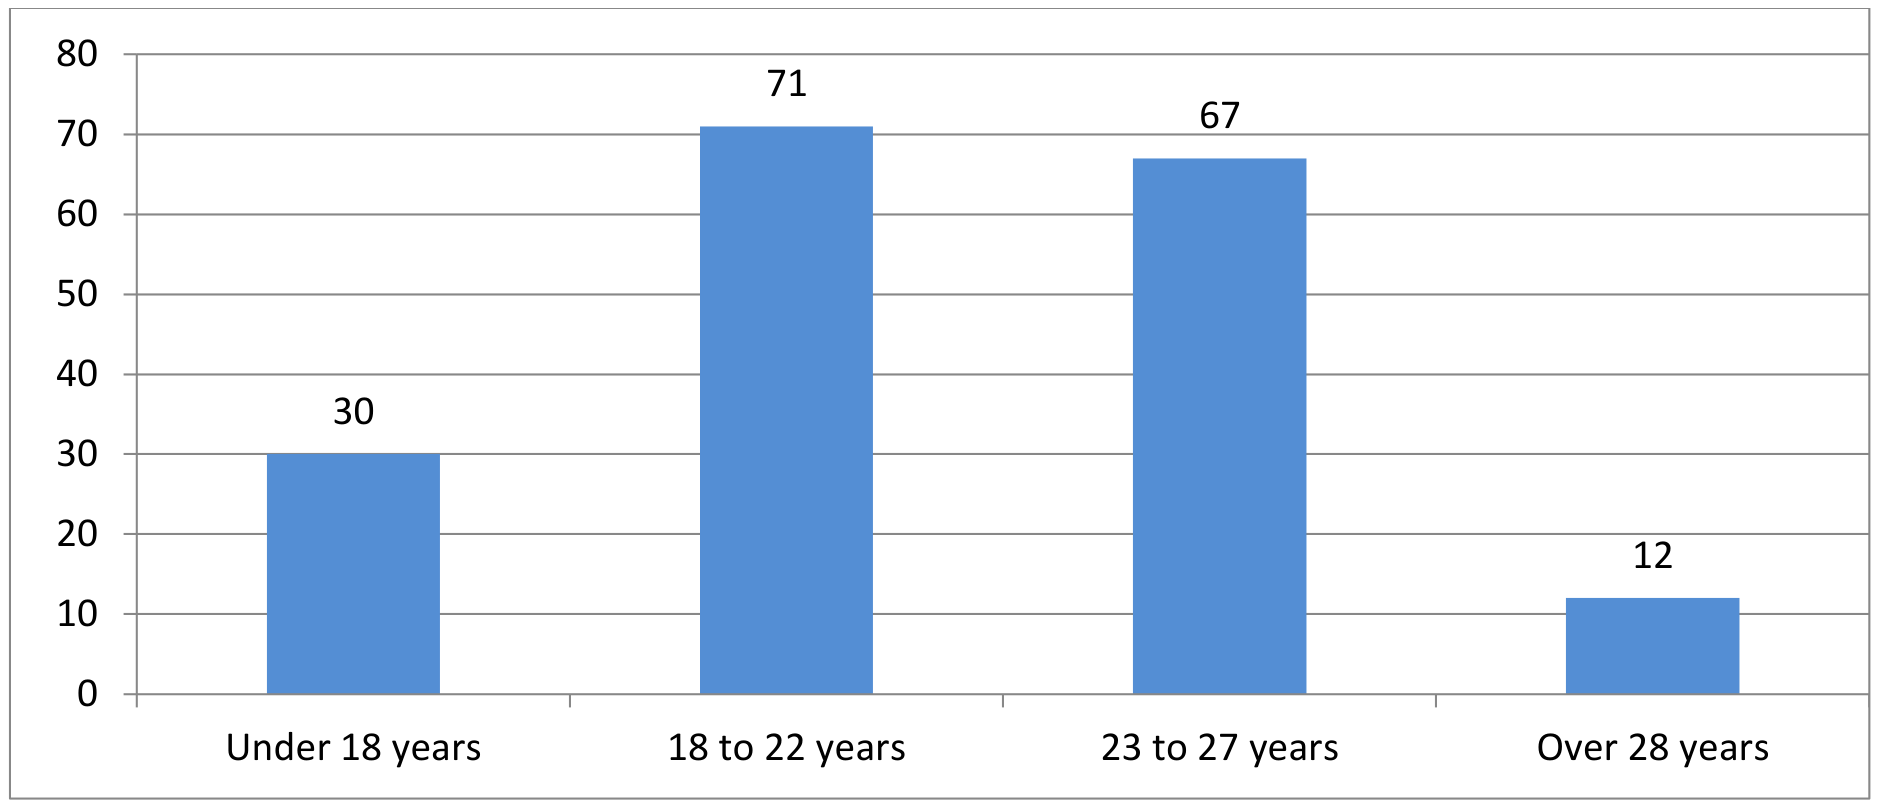
\includegraphics[width=\linewidth,height=0.3\textheight,keepaspectratio]{media/office_obj_1.png}
\caption{Sample distribution by age .}
\label{fig:office1}
\end{figure}

\begin{table*}[tbp]
\centering
{\small
\begin{tabular}{|>{\centering\arraybackslash}p{\dimexpr 0.2940\textwidth-2\tabcolsep\relax}|>{\centering\arraybackslash}p{\dimexpr 0.2560\textwidth-2\tabcolsep\relax}|>{\centering\arraybackslash}p{\dimexpr 0.1160\textwidth-2\tabcolsep\relax}|>{\centering\arraybackslash}p{\dimexpr 0.1877\textwidth-2\tabcolsep\relax}|}
\hline
\multicolumn{2}{|c|}{\cellcolor[HTML]{DDD9C3}\textbf{Variable}} & \cellcolor[HTML]{DDD9C3}\textbf{Frequency} & \cellcolor[HTML]{DDD9C3}\textbf{Percent} \\
\hline
\multirow{2}{*}{\cellcolor[HTML]{DDD9C3}Gender} & Male & 82 & 45.6\% \\
\cline{2-4}
 & Female & 98 & 54.4\% \\
\hline
\multirow{4}{*}{\cellcolor[HTML]{DDD9C3}Age} & Under 18 years & 30 & 16.7\% \\
\cline{2-4}
 & 18 to 22 years & 71 & 39.4\% \\
\cline{2-4}
 & 23 to 27 years & 67 & 37.2\% \\
\cline{2-4}
 & Over 28 years & 12 & 6.7\% \\
\hline
\multirow{5}{*}{\cellcolor[HTML]{DDD9C3}Duration} & One hour & 7 & 3.9\% \\
\cline{2-4}
 & From 1 to 3 hours & 41 & 22.8\% \\
\cline{2-4}
 & 3 to 5 hours & 84 & 46.7\% \\
\cline{2-4}
 & 5 hours or more & 48 & 26.7\% \\
\cline{2-4}
 &  & 180 & 100.0\% \\
\hline
\end{tabular}}
\caption{Table}

\end{table*}

Table 1: characteristics of the sample.

Table 1 presents the frequencies and percentages of the study sample according to gender, age, and daily duration of social media use. The results indicate that female participants constituted a slightly higher proportion of the sample (54.4\%) than male participants (45.6\%). Regarding age, the largest proportion of respondents fell within the 18–22 years age group (39.4\%), followed by those aged 23–27 years (37.2\%), while participants under 18 years and those aged 28 years or above represented 16.7\% and 6.7\% of the sample, respectively. With respect to the daily duration of social media use, nearly half of the participants (46.7\%) reported using social media for 3 to 5 hours per day. This was followed by those using social media for 5 hours or more (26.7\%) and those using it for 1 to 3 hours per day (22.8\%), whereas only 3.9\% reported using social media for one hour daily. Overall, these findings indicate that the majority of respondents spend three or more hours per day on social media platforms, reflecting a high level of daily engagement.

\begin{figure}[htbp]
\centering
\ifdim 7.1354in>\linewidth
  
\includegraphics[width=\linewidth,keepaspectratio]{media/image5.png}
\else
  
\includegraphics[width=7.1354in,height=2.7782in]{media/image5.png}
\fi
\caption{}

\end{figure}

Figure 1 shows the sample distribution according to gender.

Figure 2: Sample distribution by age.

\begin{figure}[htbp]
\centering
\ifdim 6.3646in>\linewidth
  
\includegraphics[width=\linewidth,keepaspectratio]{media/image6.png}
\else
  
\includegraphics[width=6.3646in,height=2.7708in]{media/image6.png}
\fi
\caption{}

\end{figure}

Figure 3: Daily Time Spent on Social Media by the Respondents

Figure 3 illustrates the distribution of the study sample according to the daily duration of social media use. The results indicate that the largest proportion of participants (46.7\%) reported using social media for 3 to 5 hours per day, making this the most common usage category. This was followed by participants who used social media for 5 hours or more (26.7\%), while 22.8\% reported using social media for 1 to 3 hours daily. Only 3.9\% of the participants indicated that they used social media for one hour per day. These findings suggest that the majority of the respondents spend more than three hours per day on social media platforms, reflecting a high level of exposure to online content. This supports the relevance of examining the role of social media in both the spread and prevention of electronic extremism.

\par\medskip\noindent {\large\bfseries 3.3. Sample Size Justification and Power Analysis\par}\smallskip

The sample size was considered adequate for the statistical analyses performed in this study. According to Hair et al. (2019), a sample of 150–200 participants is generally sufficient for exploratory factor analysis when sampling adequacy is satisfactory. In the present study, the Kaiser–Meyer–Olkin (KMO) value was 0.890, indicating excellent sampling adequacy and confirming that the sample was appropriate for the analyses conducted.

To further evaluate the adequacy of the sample size, a post hoc power analysis was conducted using G*Power 3.1. Based on the observed large effect size (Cohen's f = 0.631), a significance level of α = .05, four comparison groups, and a total sample of 180 participants, the achieved statistical power was 1.00, indicating that the sample size was sufficient to detect the observed effect with excellent statistical power.

\par\medskip\noindent {\large\bfseries 3.4. Data Collection Procedure\par}\smallskip

Data were collected using a structured online questionnaire created through Google Forms. The survey link was distributed electronically to students at Zayed University through commonly used communication platforms. Participation was voluntary, and respondents were informed about the purpose of the study before completing the questionnaire. Participants were assured that their responses would remain anonymous and confidential and would be used exclusively for academic research purposes. Only fully completed questionnaires were retained for statistical analysis, yielding a final sample of 180 valid responses.

\par\medskip\noindent {\large\bfseries 3.5 Research Instrument\par}\smallskip

After reviewing the theoretical frameworks and relevant literature, and examining the research instruments employed in previous studies—specifically those by Abu-Khatwa and Al-Baz (2014), Helal (2020), Al-Bulahid, Al-Firas, and Al-Taleb (2023), Al-Mughadhwi (2020), Al-Ali and Al-Ali (2017), and Al-Fuqaha (2016) and further guided by the insights and consultations of panel experts and specialists among faculty members in education, media, and educational measurement and evaluation.

Data were collected using a structured questionnaire developed to examine university students' perceptions of the role of social media in spreading and countering cyber-extremism. The questionnaire was developed after an extensive review of the relevant literature and previous empirical studies addressing social media use and cyber-extremism. The instrument consisted of two main dimensions: (1) the role of social media in spreading cyber-extremism and (2) the role of social media in countering cyber-extremism, comprising a total of 28 items, with 14 items assigned to each dimension.

Responses were measured using a five-point Likert scale ranging from 1 (Strongly Disagree) to 5 (Strongly Agree), where higher scores indicated stronger agreement with the statements. The questionnaire also included a demographic section designed to collect information on participants' gender, age, duration of social media use, and the social media platforms they used most frequently

\par\medskip\noindent {\large\bfseries 3.6. Validity and Reliability of the Instrument\par}\smallskip

Interrater validity: In the current study, face validity (expert judgment) was established by submitting the questionnaire to ten (10) referees specializing in education. They were requested to evaluate the appropriateness of the items, their relevance in terms of content and phrasing, clarity of meaning, alignment with the designated objectives, and to provide recommendations for any necessary modifications, deletions, or additions. In light of the referees’ feedback, the researcher rephrased several items and deleted those that did not reach an 80\% consensus. The agreement rate regarding the validity of the scale's items ranged between 90\% and 100\%.

Internal Consistency: The questionnaire was administered to a pilot sample consisting of ninety (90) students from Zayed University in the United Arab Emirates to calculate its psychometric properties. The following analyses were conducted: Correlation Coefficients: Pearson correlation coefficients were calculated between the score of each individual questionnaire item and the total score of the questionnaire, as illustrated in Table 2.

\begin{table*}[tbp]
\centering
{\small
\begin{tabular}{|p{\dimexpr 0.1208\textwidth-2\tabcolsep\relax}|p{\dimexpr 0.1292\textwidth-2\tabcolsep\relax}|p{\dimexpr 0.1207\textwidth-2\tabcolsep\relax}|p{\dimexpr 0.1292\textwidth-2\tabcolsep\relax}|p{\dimexpr 0.1207\textwidth-2\tabcolsep\relax}|p{\dimexpr 0.1292\textwidth-2\tabcolsep\relax}|p{\dimexpr 0.1208\textwidth-2\tabcolsep\relax}|p{\dimexpr 0.1292\textwidth-2\tabcolsep\relax}|}
\hline
\cellcolor[HTML]{DDD9C3}\textbf{Item} & \cellcolor[HTML]{DDD9C3}\textbf{Correlation Coefficient} & \cellcolor[HTML]{DDD9C3}\textbf{Item} & \cellcolor[HTML]{DDD9C3}\textbf{Correlation Coefficient} & \cellcolor[HTML]{DDD9C3}\textbf{Item} & \cellcolor[HTML]{DDD9C3}\textbf{Correlation Coefficient} & \cellcolor[HTML]{DDD9C3}\textbf{Item} & \cellcolor[HTML]{DDD9C3}\textbf{Correlation Coefficient} \\
\hline
\cellcolor[HTML]{DDD9C3}\textbf{1} & **0.639 & \textbf{8} & **0.814 & \textbf{15} & **0.666 & \textbf{22} & **0.605 \\
\hline
\cellcolor[HTML]{DDD9C3}\textbf{2} & **0.749 & \textbf{9} & **0.833 & \textbf{16} & **0.759 & \textbf{23} & **0.780 \\
\hline
\cellcolor[HTML]{DDD9C3}\textbf{3} & **0.787 & \textbf{10} & **0.734 & \textbf{17} & **0.614 & \textbf{24} & **0.661 \\
\hline
\cellcolor[HTML]{DDD9C3}\textbf{4} & **0.717 & \textbf{11} & **0.513 & \textbf{18} & **0.616 & \textbf{25} & **0.554 \\
\hline
\cellcolor[HTML]{DDD9C3}\textbf{5} & **0.488 & \textbf{12} & **0.475 & \textbf{19} & **0.793 & \textbf{26} & **0.662 \\
\hline
\cellcolor[HTML]{DDD9C3}\textbf{6} & **0.774 & \textbf{13} & **0.371 & \textbf{20} & **0.596 & \textbf{27} & **0.608 \\
\hline
\cellcolor[HTML]{DDD9C3}\textbf{7} & **0.732 & \textbf{14} & **0.404 & \textbf{21} & **0.577 & \textbf{28} & **0.478 \\
\hline
\end{tabular}}
\caption{Table}

\end{table*}

Table 2: Item-Total Correlation Coefficients of the Questionnaire

As shown in Table 2, the corrected item–total correlation coefficients ranged from 0.371 to 0.833. All coefficients exceeded the recommended minimum threshold of 0.30, indicating satisfactory internal consistency and confirming that all questionnaire items contributed adequately to measuring their respective constructs. Therefore, all items were retained for subsequent statistical analyses.

Questionnaire Reliability: The questionnaire was administered to a sample of ninety (90) students at Zayed University in the United Arab Emirates. To assess the reliability of the instrument, both Cronbach's alpha and test-retest reliability coefficients were calculated. The results are presented in Table 3 below:

\begin{table*}[tbp]
\centering
{\renewcommand{\arraystretch}{1.54}\small
\begin{tabular}{|>{\centering\arraybackslash}p{\dimexpr 0.3333\textwidth-2\tabcolsep\relax}|>{\centering\arraybackslash}p{\dimexpr 0.3333\textwidth-2\tabcolsep\relax}|>{\centering\arraybackslash}p{\dimexpr 0.3334\textwidth-2\tabcolsep\relax}|}
\hline
\cellcolor[HTML]{DDD9C3}\textbf{Test-Retest Reliability Coefficient} & \cellcolor[HTML]{DDD9C3}\textbf{Cronbach's Alpha Coefficient} & \cellcolor[HTML]{DDD9C3}\textbf{Dimensions} \\
\hline
\cellcolor[HTML]{DDD9C3}0.877 & 0.856 & Total Score \\
\hline
\end{tabular}}
\caption{Table}

\end{table*}

Table 3 : Reliability Coefficients of the Questionnaire

As shown in Table 3, the questionnaire exhibited satisfactory reliability. The overall Cronbach's alpha coefficient was 0.856, demonstrating good internal consistency among the questionnaire items. Furthermore, the test–retest reliability coefficient reached 0.877, indicating that the instrument maintained a high level of stability over time. These results provide strong evidence that the questionnaire is reliable and suitable for collecting data in the current study.

Construct Validity

To examine construct validity, an exploratory factor analysis (EFA) using Principal Component Analysis with Varimax rotation was conducted. The Kaiser–Meyer–Olkin (KMO) measure was 0.890, indicating excellent sampling adequacy, while Bartlett's Test of Sphericity was statistically significant (χ² = 3232.818, df = 378, p \textless{} .001), confirming the suitability of the data for factor analysis. Based on the theoretical framework, the number of extracted factors was fixed at two. The first factor explained 29.94\% of the total variance, whereas the second explained 21.42\%, accounting for a cumulative variance of 51.36\%. Factor loadings ranged from 0.605 to 0.825 for the first factor and from 0.421 to 0.870 for the second factor, providing satisfactory evidence of the questionnaire's construct validity. as illustrated in Table 4.

\begin{table*}[tbp]
\centering
{\small
\begin{tabular}{|>{\centering\arraybackslash}p{\dimexpr 0.4220\textwidth-2\tabcolsep\relax}|>{\centering\arraybackslash}p{\dimexpr 0.5163\textwidth-2\tabcolsep\relax}|}
\hline
\cellcolor[HTML]{DDD9C3}\textbf{Indicator} & \cellcolor[HTML]{DDD9C3}\textbf{Result} \\
\hline
\cellcolor[HTML]{DDD9C3}Kaiser–Meyer–Olkin (KMO) & 0.890 \\
\hline
\cellcolor[HTML]{DDD9C3}Bartlett's Test of Sphericity & χ² = 3232.818, df = 378, p \textless{} .001 \\
\hline
\cellcolor[HTML]{DDD9C3}Extraction Method & Principal Component Analysis (PCA) \\
\hline
\cellcolor[HTML]{DDD9C3}Rotation Method & Varimax with Kaiser Normalization \\
\hline
\cellcolor[HTML]{DDD9C3}Number of Extracted Factors & 2 (fixed according to the theoretical framework) \\
\hline
\cellcolor[HTML]{DDD9C3}Eigenvalue of Factor 1 & 8.383 \\
\hline
\cellcolor[HTML]{DDD9C3}Variance Explained by Factor 1 & 29.94\% \\
\hline
\cellcolor[HTML]{DDD9C3}Eigenvalue of Factor 2 & 5.999 \\
\hline
\cellcolor[HTML]{DDD9C3}Variance Explained by Factor 2 & 21.42\% \\
\hline
\cellcolor[HTML]{DDD9C3}Total Explained Variance & 51.36\% \\
\hline
\cellcolor[HTML]{DDD9C3}Factor Loadings (Factor 1: QP1–QP14) & 0.605–0.825 \\
\hline
\cellcolor[HTML]{DDD9C3}Factor Loadings (Factor 2: Q1–Q14) & 0.421–0.870 \\
\hline
\end{tabular}}
\caption{Table}

\end{table*}

Table 4: Exploratory Factor Analysis (EFA) Results for the Questionnaire

Note. Principal Component Analysis with Varimax rotation was performed. The number of extracted factors was fixed at two based on the theoretical structure of the questionnaire. All retained items exhibited factor loadings greater than 0.40.

\par\vspace{5.0pt}\noindent {\large\bfseries 3.7 Data Analysis\par}\vspace{5.0pt}

The collected data were analyzed using IBM SPSS Statistics (Version 22). Descriptive statistics, including frequencies, percentages, means, and standard deviations, were used to summarize the demographic characteristics of the participants and describe their responses to the study variables. Prior to conducting inferential analyses, the normality of the data distribution was examined using skewness, kurtosis, and the Kolmogorov–Smirnov and Shapiro–Wilk tests.

The psychometric properties of the questionnaire were assessed through exploratory factor analysis (EFA), Cronbach's alpha, and test–retest reliability. Independent-samples t-tests were employed to examine differences according to gender, while one-way analysis of variance (ANOVA) was used to assess differences across age groups and duration of social media use. When the assumption of homogeneity of variances was violated, the Games–Howell post hoc test was applied to identify pairwise group differences. Pearson's correlation coefficient was used to examine the relationship between the two study dimensions. In addition, effect size indices (Cohen's d and η²) were calculated to evaluate the practical significance of statistically significant findings. Statistical significance was determined at the 0.05 level.

\par\vspace{5.0pt}\noindent {\large\bfseries 4. Results\par}\vspace{5.0pt}

\par\vspace{5.0pt}\noindent {\large\bfseries 4.1 Social Media Platforms Most Frequently Used\par}\vspace{5.0pt}

To answer the first research question regarding the most frequently used social media platforms among Zayed University students, frequencies and percentages were calculated. The results are presented in Table (4) and Figure 4.

\begin{table*}[tbp]
\centering
{\small
\begin{tabular}{|p{\dimexpr 0.1370\textwidth-2\tabcolsep\relax}|p{\dimexpr 0.1982\textwidth-2\tabcolsep\relax}|p{\dimexpr 0.3296\textwidth-2\tabcolsep\relax}|}
\hline
\cellcolor[HTML]{DDD9C3}\textbf{Percent} & \cellcolor[HTML]{DDD9C3}\textbf{Frequency} & \cellcolor[HTML]{DDD9C3}\textbf{Preferred social media platform} \\
\hline
33.9\% & 61 & \cellcolor[HTML]{DDD9C3}X (formerly Twitter) \\
\hline
20.0\% & 36 & \cellcolor[HTML]{DDD9C3}TikTok \\
\hline
18.3\% & 33 & \cellcolor[HTML]{DDD9C3}Instagram \\
\hline
17.8\% & 32 & \cellcolor[HTML]{DDD9C3}Facebook \\
\hline
7.8\% & 14 & \cellcolor[HTML]{DDD9C3}Snapchat \\
\hline
2.2\% & 4 & \cellcolor[HTML]{DDD9C3}YouTube \\
\hline
100.0\% & 180 & \cellcolor[HTML]{DDD9C3}Total \\
\hline
\end{tabular}}
\caption{Table}

\end{table*}

Table 4: The Preferred social media platform

\begin{figure}[htbp]
\centering
\ifdim 6.0417in>\linewidth
  
\includegraphics[width=\linewidth,keepaspectratio]{media/image7.png}
\else
  
\includegraphics[width=6.0417in,height=3.5000in]{media/image7.png}
\fi
\caption{}

\end{figure}

Figure 4: Distribution of Respondents by Preferred Social Media Platform

Figure (4) illustrates the distribution of the study sample according to the most frequently used social media platform. The results show that X (formerly Twitter) was the most frequently used platform among the participants, accounting for 33.9\% (n = 61), followed by TikTok with 20.0\% (n = 36), Instagram with 18.3\% (n = 33), and Facebook with 17.8\% (n = 32). Snapchat ranked fifth, representing 7.8\% (n = 14) of the sample, whereas YouTube was the least frequently used platform, accounting for only 2.2\% (n = 4). These findings indicate that X (formerly Twitter) is the dominant social media platform among the study participants, suggesting that it may play a particularly influential role in shaping their exposure to online content, including issues related to electronic extremism.

4.2.Descriptive Statistics

Following the assessment of the questionnaire's validity and reliability, descriptive statistical analyses were conducted to summarize the respondents' perceptions of the study dimensions. Means and standard deviations were calculated for each dimension based on the five-point Likert scale to determine the level of respondents' perceptions.

\begin{table*}[tbp]
\centering
{\small
\begin{tabular}{|p{\dimexpr 0.2083\textwidth-2\tabcolsep\relax}|>{\centering\arraybackslash}p{\dimexpr 0.2083\textwidth-2\tabcolsep\relax}|>{\centering\arraybackslash}p{\dimexpr 0.2083\textwidth-2\tabcolsep\relax}|>{\centering\arraybackslash}p{\dimexpr 0.2877\textwidth-2\tabcolsep\relax}|}
\hline
\cellcolor[HTML]{DDD9C3}\textbf{Variable} & \cellcolor[HTML]{DDD9C3}\textbf{Mean} & \cellcolor[HTML]{DDD9C3}\textbf{Std.} & \cellcolor[HTML]{DDD9C3}\textbf{Level} \\
\hline
\cellcolor[HTML]{DDD9C3}The Spread of Cyber-Extremism & 3.32 & 0.903 & Moderate \\
\hline
\cellcolor[HTML]{DDD9C3}Combating Cyber-Extremism & 3.49 & 0.866 & High \\
\hline
\cellcolor[HTML]{DDD9C3}Overall & 3.40 & 0.577 & Moderate \\
\hline
\end{tabular}}
\caption{Table}

\end{table*}

Table 5: Means and Standard Deviations of the Study Dimensions

Table 5: presents the descriptive statistics for the study dimensions. The findings indicate that the overall mean score of the questionnaire was 3.40 (SD = 0.577), reflecting a moderate level. Among the two dimensions, Countering Electronic Extremism recorded the highest mean (M = 3.49, SD = 0.866), indicating a high level. In contrast, Spread of Electronic Extremism obtained a mean of 3.32 (SD = 0.903), representing a moderate level. These findings suggest that respondents perceived the role of social media in countering electronic extremism to be slightly stronger than its role in facilitating the spread of electronic extremism.

Prior to conducting the inferential statistical analyses, the assumption of normality was assessed by examining the skewness and kurtosis values of the study variables. The obtained skewness values ranged from −0.673 to −0.263, while the kurtosis values ranged from −1.445 to −0.062. These values fell within the acceptable ranges recommended in the methodological literature, indicating that the data were approximately normally distributed. Therefore, parametric statistical tests were deemed appropriate for testing the study hypotheses (Hair et al., 2019).

\par\vspace{5.0pt}\noindent {\large\bfseries 4.3 Differences in Perceptions of the Role of Social Media in Spreading Cyber-Extremism\par}\vspace{5.0pt}

To address the fourth research question, inferential statistical analyses were performed to examine whether respondents' perceptions of the role of social media in spreading cyber-extremism varied according to gender, age, and duration of social media use. An independent-samples t-test was conducted for gender, whereas one-way ANOVA was used for age and duration of social media use. The results are summarized in Table 6.

\begin{table*}[tbp]
\centering
{\small
\begin{tabular}{|>{\centering\arraybackslash}p{\dimexpr 0.1805\textwidth-2\tabcolsep\relax}|>{\centering\arraybackslash}p{\dimexpr 0.1775\textwidth-2\tabcolsep\relax}|>{\centering\arraybackslash}p{\dimexpr 0.1782\textwidth-2\tabcolsep\relax}|p{\dimexpr 0.1476\textwidth-2\tabcolsep\relax}|>{\centering\arraybackslash}p{\dimexpr 0.3162\textwidth-2\tabcolsep\relax}|}
\hline
\cellcolor[HTML]{DDD9C3}\textbf{Demographic Variable} & \cellcolor[HTML]{DDD9C3}\textbf{Statistical Test} & \cellcolor[HTML]{DDD9C3}\textbf{Test Statistic} & \cellcolor[HTML]{DDD9C3}\textbf{p-value} & \cellcolor[HTML]{DDD9C3}\textbf{Decision} \\
\hline
\cellcolor[HTML]{DDD9C3}\textbf{Gender} & Independent-samples t-test & t(178) = 0.384 & .701 & Not Significant \\
\hline
\cellcolor[HTML]{DDD9C3}\textbf{Age} & One-way ANOVA & F(3,176) = 1.113 & .345 & Not Significant \\
\hline
\cellcolor[HTML]{DDD9C3}\textbf{Duration of Social Media Use} & One-way ANOVA & F(3,176) = 2.543 & .058 & Not Significant \\
\hline
\end{tabular}}
\caption{Table}

\end{table*}

Table 6: Differences in Respondents' Perceptions of the Role of Social Media in Spreading Cyber-Extremism According to Demographic Variables.

Table 6: presents the results of the inferential analyses examining differences in respondents' perceptions of the role of social media in spreading cyber-extremism according to demographic variables. The independent-samples t-test indicated that there were no statistically significant differences between male and female respondents, t(178) = 0.384, p = .701. Likewise, the one-way ANOVA showed no statistically significant differences across age groups, F(3,176) = 1.113, p = .345, or according to the duration of social media use, F(3,176) = 2.543, p = .058. Therefore, respondents' perceptions of the role of social media in spreading cyber-extremism were consistent across all demographic categories examined.

\par\medskip\noindent {\large\bfseries 4.4 Differences in Perceptions of the Role of Social Media in Countering Cyber-Extremism\par}\smallskip

To answer the fifth research question—Are there statistically significant differences in respondents' perceptions of the role of social media in countering cyber-extremism attributable to gender, age, and duration of social media use?—inferential statistical analyses were conducted. An independent-samples t-test was used to compare respondents' perceptions by gender, while one-way analysis of variance (ANOVA) was employed to examine differences across age groups and duration of social media use. The findings are summarized in Table 7.

\begin{table*}[tbp]
\centering
{\small
\begin{tabular}{|>{\centering\arraybackslash}p{\dimexpr 0.1739\textwidth-2\tabcolsep\relax}|>{\centering\arraybackslash}p{\dimexpr 0.1710\textwidth-2\tabcolsep\relax}|>{\centering\arraybackslash}p{\dimexpr 0.1991\textwidth-2\tabcolsep\relax}|p{\dimexpr 0.1368\textwidth-2\tabcolsep\relax}|>{\centering\arraybackslash}p{\dimexpr 0.2326\textwidth-2\tabcolsep\relax}|}
\hline
\cellcolor[HTML]{DDD9C3}\textbf{Demographic Variable} & \cellcolor[HTML]{DDD9C3}\textbf{Statistical Test} & \cellcolor[HTML]{DDD9C3}\textbf{Test Statistic} & \cellcolor[HTML]{DDD9C3}\textbf{p-value} & \cellcolor[HTML]{DDD9C3}\textbf{Decision} \\
\hline
\cellcolor[HTML]{DDD9C3}\textbf{Gender} & Independent-samples t-test & t(178) = 0.578 & .564 & Not Significant \\
\hline
\cellcolor[HTML]{DDD9C3}\textbf{Age} & One-way ANOVA & F(3,176) = 23.373 & \textless{} .001 & Significant \\
\hline
\cellcolor[HTML]{DDD9C3}\textbf{Duration of Social Media Use} & One-way ANOVA & F(3,176) = 2.445 & .066 & Not Significant \\
\hline
\end{tabular}}
\caption{Table}

\end{table*}

Table 7: Differences in respondents' perceptions of the role of social media in countering cyber-extremism according to demographic variables

Table 7: presents the results of the inferential analyses examining differences in respondents' perceptions of the role of social media in countering cyber-extremism according to demographic variables. The findings revealed that gender and duration of social media use did not produce statistically significant differences in respondents' perceptions (p \textgreater{} .05). In contrast, statistically significant differences were observed across age groups (F(3,176) = 23.373, p \textless{} .001). Post hoc Games–Howell comparisons indicated that the 23–27-year age group reported significantly higher perceptions than the remaining age groups, whereas no significant difference was found between participants aged under 18 years and those aged 28 years and above.

\par\medskip\noindent {\large\bfseries 4.5 Relationship Between the Study Variables\par}\smallskip

To answer the sixth research question, which examined whether there is a statistically significant relationship between respondents' perceptions of the role of social media in spreading cyber-extremism and their perceptions of its role in countering cyber-extremism, Pearson's product-moment correlation analysis was conducted. The results are presented in Table 8.

\begin{table*}[tbp]
\centering
{\small
\begin{tabular}{|p{\dimexpr 0.1643\textwidth-2\tabcolsep\relax}|p{\dimexpr 0.1643\textwidth-2\tabcolsep\relax}|p{\dimexpr 0.1643\textwidth-2\tabcolsep\relax}|p{\dimexpr 0.1643\textwidth-2\tabcolsep\relax}|p{\dimexpr 0.2291\textwidth-2\tabcolsep\relax}|}
\hline
\cellcolor[HTML]{DDD9C3}\textbf{Variable} & \cellcolor[HTML]{DDD9C3}\textbf{Correlation (S)} & \cellcolor[HTML]{DDD9C3}\textbf{Sig.} & \cellcolor[HTML]{DDD9C3}\textbf{Correlation (CO)} & \cellcolor[HTML]{DDD9C3}\textbf{Sig.} \\
\hline
\cellcolor[HTML]{DDD9C3}S & — & — & −0.152* & 0.042 \\
\hline
\cellcolor[HTML]{DDD9C3}CO & — & — & — & — \\
\hline
\end{tabular}}
\caption{Table}

\end{table*}

Table 8 Pearson correlation between perceptions of the role of social media in spreading and countering cyber-extremism.

Note. N = 180. p \textless{} .05 (two-tailed).

Pearson's product-moment correlation analysis was conducted to examine the relationship between respondents' perceptions of the role of social media in spreading cyber-extremism and their perceptions of its role in countering cyber-extremism. As shown in Table X, a weak negative correlation was found between the two variables (r = −0.152, p = .042). Although the relationship was statistically significant, its magnitude was small, indicating that respondents who perceived social media as playing a greater role in spreading cyber-extremism tended to report slightly lower perceptions of its role in countering cyber-extremism.

To complement the statistical significance tests, effect sizes were calculated to evaluate the practical significance of the findings. The results indicated negligible effect sizes for gender differences in both the perceived role of social media in spreading cyber-extremism (Cohen's d = 0.06) and countering cyber-extremism (Cohen's d = 0.09). Regarding age, a small effect size was observed for perceptions of social media's role in spreading cyber-extremism (η² = 0.042), whereas a large effect size was found for perceptions of its role in countering cyber-extremism (η² = 0.285), indicating that age accounted for approximately 28.5\% of the variance in respondents' perceptions. In contrast, the duration of social media use demonstrated a small effect size (η² = 0.040). Finally, the statistically significant correlation between the two study variables represented a weak negative association (r = −0.152). These findings suggest that, although some statistically significant relationships were identified, their practical significance varied across the examined demographic variables.

\par\medskip\noindent {\large\bfseries 5. Discussion\par}\smallskip

The findings showed that X (formerly Twitter) was the most frequently used social media platform among Zayed University students, followed by TikTok and Instagram. This pattern reflects students' preference for highly interactive platforms that facilitate rapid information exchange and public engagement. Given the widespread use of these platforms, they represent important digital spaces where both constructive communication and exposure to extremist content may occur. This finding is consistent with previous studies highlighting that social media has become a primary environment through which extremist organizations disseminate propaganda and interact with online audiences (Awan, 2017; Antonova, 2023).

The findings revealed that respondents perceived social media as playing a stronger role in countering cyber-extremism than in facilitating its spread. This suggests that university students recognize the increasing efforts undertaken by digital platforms to limit extremist content through content moderation, reporting systems, and algorithm-based detection technologies. Such efforts may have strengthened users' confidence in the preventive role of social media while acknowledging that extremist actors continue to exploit these platforms to disseminate radical narratives. This interpretation is consistent with recent studies indicating that social media companies have expanded their technological and policy-based measures to detect, remove, and restrict extremist content, while simultaneously enhancing cooperation with governmental and civil society initiatives aimed at countering online extremism (Weimann \& Masri, 2023; Tahat et al., 2024). Nevertheless, the findings also indicate that these technological interventions have not entirely eliminated the risks associated with cyber-extremism. The continued moderate perception of social media's role in facilitating extremism suggests that technological mechanisms, including algorithmic content recommendation and the rapid dissemination of online information, remain ongoing challenges despite recent advances in platform governance.

The findings indicated that respondents' perceptions of the role of social media in spreading cyber-extremism did not differ significantly according to gender, age, or duration of social media use. Similarly, no significant differences were observed according to gender or duration of use in relation to the perceived role of social media in countering cyber-extremism. These findings suggest that awareness of cyber-extremism is relatively consistent among university students regardless of gender or patterns of social media use. This result is consistent with previous studies reporting that the widespread integration of social media into students' daily lives has reduced demographic differences in digital engagement and exposure to online content (Hilal, 2020; Al-Saray, 2025)

In contrast, statistically significant differences were found across age groups regarding perceptions of the role of social media in countering cyber-extremism, with participants aged 23–27 years reporting higher levels of awareness than the other age groups. This finding may be explained by the greater academic maturity and broader digital experience of older students, which may enhance their ability to recognize both the risks of extremist content and the importance of preventive measures. This interpretation is consistent with studies emphasizing the role of universities in strengthening intellectual security and developing students' critical awareness of digital risks (Solerem, 2025). The findings therefore suggest that age, rather than gender or duration of social media use, represents the demographic factor most closely associated with students' perceptions of efforts to counter cyber-extremism.

Finally, the study identified a statistically significant but weak negative relationship between students' perceptions of the role of social media in spreading cyber-extremism and its role in countering it. This finding suggests that respondents who perceived social media as more influential in facilitating cyber-extremism tended to express slightly lower confidence in its capacity to counter extremist activities. Although the relationship was weak, it reflects students' awareness that the same digital platforms can simultaneously serve as channels for extremist exploitation and as tools for prevention. This perception may stem from the rapid dissemination of online content, which often challenges the effectiveness of preventive measures despite continuous technological improvements (Binder \& Kenyon, 2022; Tahat et al., 2024).

From an educational perspective, these findings indicate that combating cyber-extremism should not rely exclusively on technological interventions or platform moderation. Rather, strengthening digital citizenship, critical thinking, and media and information literacy is essential for enabling young people to critically assess online content and resist extremist narratives (Hobbs, 2017; Frau-Meigs, 2019).

From an Islamic jurisprudential perspective, the findings further suggest that combating cyber-extremism cannot be achieved solely through the removal of harmful online content after its dissemination. Instead, greater emphasis should be placed on cultivating ethical awareness, sound intellectual judgment, and responsible digital behaviour before exposure to extremist narratives occurs. This preventive approach is fully aligned with the objectives of Islamic Sharia, which prioritize preventing harm before it occurs and safeguarding religion, intellect, and social stability through proactive educational and ethical guidance (Attia, 2021; Musa, 2025).

\par\medskip\noindent {\large\bfseries 6. Practical Implications\par}\smallskip

The findings of this study have several practical implications for universities, policymakers, and social media platforms. First, universities should strengthen digital citizenship and media literacy programmes to enhance students' ability to critically evaluate online information and recognize extremist narratives before they influence attitudes or behaviours. Particular attention should be directed toward younger university students, as the findings indicated lower levels of perceived awareness regarding the role of social media in countering cyber-extremism.

Second, social media platforms should continue improving algorithmic monitoring, content moderation, and reporting mechanisms to reduce the visibility and dissemination of extremist material while preserving opportunities for legitimate public engagement. Given that participants acknowledged both the preventive and risk-related roles of social media, technological interventions should be accompanied by transparent governance and continuous evaluation of platform policies.

Finally, the findings support closer collaboration between universities, governmental institutions, religious authorities, and social media companies in developing integrated strategies for preventing cyber-extremism. Such cooperation should combine technological safeguards with educational initiatives and ethical guidance to strengthen intellectual security and promote responsible digital participation among university students.

\par\medskip\noindent {\large\bfseries 7. Limitations of the stydy\par}\smallskip

This study was conducted among students from a single university in the United Arab Emirates, which may limit the generalizability of the findings to students in other higher education institutions or cultural contexts. Future studies are encouraged to include multiple universities from different regions to enhance the external validity of the findings.

\par\medskip\noindent {\large\bfseries 8. Recommendations for Future Research\par}\smallskip

Future research should examine cyber-extremism across a wider range of universities and cultural settings to enhance the generalizability of the findings. Longitudinal studies are also recommended to investigate how students' perceptions of cyber-extremism evolve over time and in response to changes in social media platforms and counter-extremism policies. In addition, future studies may employ qualitative or mixed-methods approaches to gain deeper insights into the motivations, experiences, and online behaviours associated with exposure to extremist content. Finally, further research is encouraged to evaluate the effectiveness of educational programmes based on digital citizenship and Islamic ethical principles in strengthening students' resilience against online radicalization.

\begin{thebibliography}{99}
\bibitem{ref1}
M.S.H. Al-Balhaid, M.S.Y. Al-Firas, B.A.F. Al-Talib, The role of social networks in intellectual extremism from the perspective of Jouf University female students and its relationship with a number of variables, Journal of Educational and Qualitative Research 17, 1–126 (2023).

\bibitem{ref2}
E.Y. Antonova, Terrorist crimes in the era of digitalization: Forms of activity and measures for counteraction, Journal of Digital Technologies and Law 11 (2023).

\bibitem{ref3}
R.A. Al-Awadhi, Al-Mughni fi Fiqh Wasa'il al-Tawasul al-Ijtima'i [The Sufficient Book in the Jurisprudence of Social Media], 1438 AH (2017).

\bibitem{ref4}
M.S. Al-Ghamdi, The major jurisprudential maxims related to social media, Journal of Arabic Studies, Faculty of Dar Al-Uloom, Minia University (2020).

\bibitem{ref5}
A.A.A. Al-Maghdhawi, Activating the role of social media sites in confronting intellectual extremism from the experts' perspective, Journal of the Islamic University for Educational and Social Sciences 1 (2020).

\bibitem{ref6}
A.Z.D. Al-Sarai, The role of social media sites in limiting the spread of intellectual extremism among university students, Wasit Journal for Human Sciences 21(3) (2025).

\bibitem{ref7}
E.A. Abu Khatwa, A.N.A. Al-Baz, Social networking and its effects on the intellectual security of university students in the Kingdom of Bahrain, The Arab Journal for Quality Assurance in Higher Education 7(15), 187–225 (2014).

\bibitem{ref8}
I. Awan, Cyber-Extremism: ISIS and the Power of Social Media, Society 54, 138–149 (2017).

\bibitem{ref9}
F.M. Attia, Social media in the balance of Sharia objectives (Maqasid), Ibn Khaldun Journal for Studies and Research 2(4), 59–83 (2021).

\bibitem{ref10}
M.F. Bastug, A. Douai, D. Akca, Exploring the demand side of online radicalization: Evidence from the Canadian context, Studies in Conflict \& Terrorism 43(7), 616–637 (2020).

\bibitem{ref11}
J.F. Binder, J. Kenyon, Terrorism and the internet: How dangerous is online radicalization? Frontiers in Psychology 13, 997390 (2022).

\bibitem{ref12}
M. Cinelli, G. De Francisci Morales, A. Galeazzi, W. Quattrociocchi, M. Starnini, The echo chamber effect on social media, Proceedings of the National Academy of Sciences 118(9), e2023301118 (2021).

\bibitem{ref13}
D. Correa, A. Sureka, Solutions to detect and analyze online radicalization: A survey, arXiv preprint, arXiv:1301.4916 (2013).

\bibitem{ref14}
M. Conway, Determining the role of the internet in violent extremism and terrorism: Six suggestions for progressing research, Studies in Conflict \& Terrorism 40(1), 77–98 (2017).

\bibitem{ref15}
G. Cascavilla, D.A. Tamburri, F. Leotta, M. Mecella, W. Van Den Heuvel, Counterterrorism in cyber-physical spaces: Best practices and technologies from state of the art, Information and Software Technology 161, 107260 (2023).

\bibitem{ref16}
C.K. Ebbrecht, R.A. Peters, Radical digital lives: Mechanisms in online radicalization and perspectives on prevention, Psyke \& Logos 45(1), 143–169 (2024).

\bibitem{ref17}
C.K. Ebbrecht, Systematic review: Risk factors and mechanisms of radicalization in lone-actor grievance-fueled violence, Nordic Psychology (2022).

\bibitem{ref18}
G. Hassan, S. Brouillette-Alarie, S. Alava, D. Frau-Meigs, L. Lavoie, A. Fetiu, S. Sieckelinck, Exposure to extremist online content could lead to violent radicalization: A systematic review of empirical evidence, International Journal of Developmental Science 12(1–2), 71–88 (2018).

\bibitem{ref19}
R. Hobbs, Create to Learn: Introduction to Digital Literacy, John Wiley \& Sons, Hoboken, NJ (2017).

\bibitem{ref20}
D. Frau-Meigs, B. O'Neill, A. Soriani, V. Tomé, Digital Citizenship Education: Overview and New Perspectives, Vol. 1, Council of Europe Publishing, Strasbourg (2017).

\bibitem{ref21}
D. Frau-Meigs, Information disorders: Risks and opportunities for digital media and information literacy, Medijske Studije 10(19), 10–28 (2019).

\bibitem{ref22}
C. Herath, J. Whittaker, Online radicalisation: Moving beyond a simple dichotomy, Terrorism and Political Violence 35(5), 1027–1048 (2023).

\bibitem{ref23}
J.F. Hair, W.C. Black, B.J. Babin, R.E. Anderson, Multivariate Data Analysis, 8th ed., Cengage Learning, Boston, MA (2019).

\bibitem{ref24}
M.A. Hilal, The impact of social networks on the attitudes and values of university students, Rawafed Journal for Scientific Studies and Research 4(2), 151–175 (2020).

\bibitem{ref25}
H.J. Ingram, An analysis of Islamic State's Dabiq magazine, Australian Journal of Political Science 51(3), 458–477 (2016).

\bibitem{ref26}
K.M. Jafar, Jurisprudence of dealing with social media sites and its effects on preserving the objectives of Islamic Sharia: A Maqasidi jurisprudential study, The Legal Journal, Faculty of Law, Cairo University 8(12), 4023–4100 (2020).

\bibitem{ref27}
J. Klausen, C. Marks, T. Zaman, Finding online extremists in social networks, arXiv preprint, arXiv:1610.06242 (2016).

\bibitem{ref28}
A. Meleagrou-Hitchens, N. Kaderbhai, Research Perspectives on Online Radicalisation: A Literature Review, 2006–2016, VOX-Pol Network of Excellence, Dublin (2017).

\bibitem{ref29}
A.M.A. Musa, Fundamentalist maxims (Usuli rules) and their relationship to regulating social media, Journal of the Faculty of Islamic and Arabic Studies for Girls in Kafr El-Sheikh 9(1) (2025).

\bibitem{ref30}
G.N. Mølmen, J.A. Ravndal, Mechanisms of online radicalisation: How the internet affects the radicalisation of extreme-right lone actor terrorists, Behavioral Sciences of Terrorism and Political Aggression 15(4), 463–487 (2023).

\bibitem{ref31}
P.R. Neumann, Options and strategies for countering online radicalization in the United States, Studies in Conflict \& Terrorism 36(6), 431–459 (2013).

\bibitem{ref32}
M. Ribble, Digital Citizenship in Schools: Nine Elements All Students Should Know, 3rd ed., International Society for Technology in Education, Washington, DC (2015).

\bibitem{ref33}
M. Risius, K.M. Blasiak, S. Wibisono, W.R. Louis, The digital augmentation of extremism: Reviewing and guiding online extremism research from a sociotechnical perspective, Information Systems Journal 34(3), 931–963 (2024).

\bibitem{ref34}
M.H. Ribeiro, R. Ottoni, R. West, V.A. Almeida, W. Meira Jr., Auditing radicalization pathways on YouTube, Proceedings of the 2020 Conference on Fairness, Accountability, and Transparency, 131–141 (2020).

\bibitem{ref35}
M. Sageman, The next generation of terror, Foreign Policy 165, 37 (2008).

\bibitem{ref36}
O. Solerem, The role of universities in promoting intellectual security: A study on a sample of University of South Africa students, Intercontinental Journal of Social Sciences 2(3), 102–114 (2025).

\bibitem{ref37}
K. Tahat, M. Habes, A. Mansoori, N. Naqbi, N. Al Ketbi, I. Maysari, A. Altawil, Social media algorithms in countering cyber extremism: A systematic review, Journal of Infrastructure, Policy and Development 8(8), 6632 (2024).

\bibitem{ref38}
I. Von Behr, A. Reding, C. Edwards, L. Gribbon, Radicalisation in the Digital Era: The Use of the Internet in 15 Cases of Terrorism and Extremism, RAND Europe, Cambridge (2013).

\bibitem{ref39}
G. Weimann, N. Masri, Research note: Spreading hate on TikTok, Studies in Conflict \& Terrorism 46(5), 752–765 (2023).

\bibitem{ref40}
C. Winter, P. Neumann, A. Meleagrou-Hitchens, M. Ranstorp, L. Vidino, J. Fürst, Online extremism: Research trends in internet activism, radicalization, and counter-strategies, International Journal of Conflict and Violence 14, 1–20 (2020).

\bibitem{ref41}
C. Winter, Documenting the Virtual Caliphate, Quilliam Foundation, London (2016).

\bibitem{ref42}
J. Whittaker, Online Radicalisation: What We Know, ResearchGate Report (2023).

\end{thebibliography}




\begin{biographyps}{media/image8.jpeg}{Dr. Amal}
Dr. Amal Salem Bashib is an Assistant Professor at Zayed University, Abu Dhabi, United Arab Emirates. She holds a PhD in Islamic Sharia (Fiqh) from Al Wasl University, Dubai. Her research interests encompass Islamic jurisprudence, family and social studies, quality of life, higher education, the ethics and applications of artificial intelligence, and contemporary Islamic issues. She has published numerous scholarly articles in her areas of expertise and has contributed to research and academic initiatives addressing contemporary societal challenges from both scientific and Islamic perspectives. She actively participates in national and international conferences and is particularly interested in advancing the integration of artificial intelligence into education and research within the framework of the objectives of Islamic law (Maqasid al-Sharia).In addition to her academic career, Dr. Bashib is a certified professional trainer, family consultant, and researcher specializing in human development and quality of life. She has extensive experience in designing and delivering professional training programs and leading community initiatives aimed at empowering families and promoting social cohesion.\end{biographyps}

\begin{biographyps}{media/image9.jpeg}{Dr. Noura}
Dr. Noura Al Naqbi is an Emirati academic and researcher specializing in educational leadership and educational technology, holding a Ph.D. in Leadership and Management. She has over 23 years of experience in education, training, and professional development. Currently, she serves as a faculty member at the Emirates College for Advanced Education (ECAE) in the Department of Education, Technology, and Teacher Preparation, specializing in Curriculum, Instruction, and Educational Technology.She is recognized for her expertise in supervising field training for teachers and educational leaders, quality assurance, evaluating educational programs, and her membership in the Research Ethics Committee. Dr. Al Naqbi has delivered numerous training programs and participated in scientific conferences both locally and internationally. She has also published research contributions in the fields of educational technology, communication, and educational innovation, and actively participates in academic committees and the development of educational initiatives supporting digital transformation and institutional excellence.\end{biographyps}

\begin{biographyps}{media/image10.jpeg}{Dr. Fatima}
Dr. Fatima Saleh AlBlooshi is an educator, researcher, and academic leader with over two decades of experience in education and higher education. She joined Zayed University in 2017, where she teaches undergraduate courses in Islamic Studies, Emirati Studies, Arabic for Non-Native Speakers, and experiential learning. Her research interests encompass education, Islamic studies, curriculum development, educational technology, and innovative teaching and learning practices. Dr. AlBlooshi has held several academic leadership roles, including Assistant Head of the Department of Islamic World Studies and Coordinator of the Islamic Civilization course, contributing to curriculum enhancement, faculty collaboration, and student success initiatives. She has published peer-reviewed articles in reputable international journals and presented her research at national and international conferences..\end{biographyps}



\end{document}
